\documentclass[11pt]{article}
\newcommand{\tablelang}{en}
% Shared preamble for paper/manuscript/tex/{en,uk}/main.tex (XeLaTeX via Tectonic).
% Layout copied from the author's FFT preprint (Zenodo 23375871) so both papers share one house style.
% The including file sets \mainlang{english} or \mainlang{ukrainian} before % Shared preamble for paper/manuscript/tex/{en,uk}/main.tex (XeLaTeX via Tectonic).
% Layout copied from the author's FFT preprint (Zenodo 23375871) so both papers share one house style.
% The including file sets \mainlang{english} or \mainlang{ukrainian} before % Shared preamble for paper/manuscript/tex/{en,uk}/main.tex (XeLaTeX via Tectonic).
% Layout copied from the author's FFT preprint (Zenodo 23375871) so both papers share one house style.
% The including file sets \mainlang{english} or \mainlang{ukrainian} before \input{../preamble}.
\usepackage[a4paper,margin=25mm]{geometry}
\usepackage{fontspec}
\setmainfont{cmunrm.otf}[BoldFont=cmunbx.otf,ItalicFont=cmunti.otf,BoldItalicFont=cmunbi.otf]
\setsansfont{cmunss.otf}[BoldFont=cmunsx.otf,ItalicFont=cmunsi.otf]
\setmonofont{cmuntt.otf}[BoldFont=cmuntb.otf,ItalicFont=cmunit.otf]
\usepackage[ukrainian,english]{babel}
\usepackage{amsmath,amssymb,amsthm,mathtools}
\usepackage{booktabs,tabularx,array,multirow}
\usepackage{graphicx}
\usepackage[font=small,labelfont=bf]{caption}
\usepackage{subcaption}
\usepackage{xcolor}
\usepackage{enumitem}
\usepackage{microtype}
\usepackage[numbers,sort&compress]{natbib}
\PassOptionsToPackage{hyphens}{url}
\usepackage[hidelinks]{hyperref}
\usepackage[nameinlink,capitalise,noabbrev]{cleveref}
\usepackage{url}
\usepackage{etoolbox}
\AtBeginEnvironment{thebibliography}{\raggedright}

\graphicspath{{../../figures/}{../../generated/figures/}}
% primitive input: LaTeX's \input is not expandable and breaks inside tabular after \midrule
\makeatletter\newcommand{\gentable}[1]{\@@input ../tables/\tablelang/T#1.tex }\makeatother

% notation (archive-index paper)
\newcommand{\code}[1]{\texttt{#1}}
\newcommand{\sys}[1]{\textsf{#1}}          % system names in tables and text: \sys{adaptive}
\newcommand{\metric}[1]{\mathrm{#1}}       % nDCG@10 etc. in math
\newcommand{\uapar}{UA-PAR}
% \pending{...}: text not written yet. Visible in the PDF; paper/release/compliance.py rejects any PDF that has one.
\newcommand{\pending}[1]{\textcolor{red}{[PENDING: #1]}}

% theorem names: the including file may define these before \input{../preamble}
\providecommand{\lemmaname}{Lemma}
\providecommand{\propositionname}{Proposition}
\providecommand{\definitionname}{Definition}
\providecommand{\remarkname}{Remark}
\providecommand{\corollaryname}{Corollary}
\providecommand{\theoremname}{Theorem}
\theoremstyle{plain}
\newtheorem{lemma}{\lemmaname}
\newtheorem{proposition}{\propositionname}
\theoremstyle{definition}
\newtheorem{definition}{\definitionname}
\theoremstyle{remark}
\newtheorem{remark}{\remarkname}

\setlength{\tabcolsep}{4pt}
\renewcommand{\arraystretch}{1.12}
\sloppy
.
\usepackage[a4paper,margin=25mm]{geometry}
\usepackage{fontspec}
\setmainfont{cmunrm.otf}[BoldFont=cmunbx.otf,ItalicFont=cmunti.otf,BoldItalicFont=cmunbi.otf]
\setsansfont{cmunss.otf}[BoldFont=cmunsx.otf,ItalicFont=cmunsi.otf]
\setmonofont{cmuntt.otf}[BoldFont=cmuntb.otf,ItalicFont=cmunit.otf]
\usepackage[ukrainian,english]{babel}
\usepackage{amsmath,amssymb,amsthm,mathtools}
\usepackage{booktabs,tabularx,array,multirow}
\usepackage{graphicx}
\usepackage[font=small,labelfont=bf]{caption}
\usepackage{subcaption}
\usepackage{xcolor}
\usepackage{enumitem}
\usepackage{microtype}
\usepackage[numbers,sort&compress]{natbib}
\PassOptionsToPackage{hyphens}{url}
\usepackage[hidelinks]{hyperref}
\usepackage[nameinlink,capitalise,noabbrev]{cleveref}
\usepackage{url}
\usepackage{etoolbox}
\AtBeginEnvironment{thebibliography}{\raggedright}

\graphicspath{{../../figures/}{../../generated/figures/}}
% primitive input: LaTeX's \input is not expandable and breaks inside tabular after \midrule
\makeatletter\newcommand{\gentable}[1]{\@@input ../tables/\tablelang/T#1.tex }\makeatother

% notation (archive-index paper)
\newcommand{\code}[1]{\texttt{#1}}
\newcommand{\sys}[1]{\textsf{#1}}          % system names in tables and text: \sys{adaptive}
\newcommand{\metric}[1]{\mathrm{#1}}       % nDCG@10 etc. in math
\newcommand{\uapar}{UA-PAR}
% \pending{...}: text not written yet. Visible in the PDF; paper/release/compliance.py rejects any PDF that has one.
\newcommand{\pending}[1]{\textcolor{red}{[PENDING: #1]}}

% theorem names: the including file may define these before % Shared preamble for paper/manuscript/tex/{en,uk}/main.tex (XeLaTeX via Tectonic).
% Layout copied from the author's FFT preprint (Zenodo 23375871) so both papers share one house style.
% The including file sets \mainlang{english} or \mainlang{ukrainian} before \input{../preamble}.
\usepackage[a4paper,margin=25mm]{geometry}
\usepackage{fontspec}
\setmainfont{cmunrm.otf}[BoldFont=cmunbx.otf,ItalicFont=cmunti.otf,BoldItalicFont=cmunbi.otf]
\setsansfont{cmunss.otf}[BoldFont=cmunsx.otf,ItalicFont=cmunsi.otf]
\setmonofont{cmuntt.otf}[BoldFont=cmuntb.otf,ItalicFont=cmunit.otf]
\usepackage[ukrainian,english]{babel}
\usepackage{amsmath,amssymb,amsthm,mathtools}
\usepackage{booktabs,tabularx,array,multirow}
\usepackage{graphicx}
\usepackage[font=small,labelfont=bf]{caption}
\usepackage{subcaption}
\usepackage{xcolor}
\usepackage{enumitem}
\usepackage{microtype}
\usepackage[numbers,sort&compress]{natbib}
\PassOptionsToPackage{hyphens}{url}
\usepackage[hidelinks]{hyperref}
\usepackage[nameinlink,capitalise,noabbrev]{cleveref}
\usepackage{url}
\usepackage{etoolbox}
\AtBeginEnvironment{thebibliography}{\raggedright}

\graphicspath{{../../figures/}{../../generated/figures/}}
% primitive input: LaTeX's \input is not expandable and breaks inside tabular after \midrule
\makeatletter\newcommand{\gentable}[1]{\@@input ../tables/\tablelang/T#1.tex }\makeatother

% notation (archive-index paper)
\newcommand{\code}[1]{\texttt{#1}}
\newcommand{\sys}[1]{\textsf{#1}}          % system names in tables and text: \sys{adaptive}
\newcommand{\metric}[1]{\mathrm{#1}}       % nDCG@10 etc. in math
\newcommand{\uapar}{UA-PAR}
% \pending{...}: text not written yet. Visible in the PDF; paper/release/compliance.py rejects any PDF that has one.
\newcommand{\pending}[1]{\textcolor{red}{[PENDING: #1]}}

% theorem names: the including file may define these before \input{../preamble}
\providecommand{\lemmaname}{Lemma}
\providecommand{\propositionname}{Proposition}
\providecommand{\definitionname}{Definition}
\providecommand{\remarkname}{Remark}
\providecommand{\corollaryname}{Corollary}
\providecommand{\theoremname}{Theorem}
\theoremstyle{plain}
\newtheorem{lemma}{\lemmaname}
\newtheorem{proposition}{\propositionname}
\theoremstyle{definition}
\newtheorem{definition}{\definitionname}
\theoremstyle{remark}
\newtheorem{remark}{\remarkname}

\setlength{\tabcolsep}{4pt}
\renewcommand{\arraystretch}{1.12}
\sloppy

\providecommand{\lemmaname}{Lemma}
\providecommand{\propositionname}{Proposition}
\providecommand{\definitionname}{Definition}
\providecommand{\remarkname}{Remark}
\providecommand{\corollaryname}{Corollary}
\providecommand{\theoremname}{Theorem}
\theoremstyle{plain}
\newtheorem{lemma}{\lemmaname}
\newtheorem{proposition}{\propositionname}
\theoremstyle{definition}
\newtheorem{definition}{\definitionname}
\theoremstyle{remark}
\newtheorem{remark}{\remarkname}

\setlength{\tabcolsep}{4pt}
\renewcommand{\arraystretch}{1.12}
\sloppy
.
\usepackage[a4paper,margin=25mm]{geometry}
\usepackage{fontspec}
\setmainfont{cmunrm.otf}[BoldFont=cmunbx.otf,ItalicFont=cmunti.otf,BoldItalicFont=cmunbi.otf]
\setsansfont{cmunss.otf}[BoldFont=cmunsx.otf,ItalicFont=cmunsi.otf]
\setmonofont{cmuntt.otf}[BoldFont=cmuntb.otf,ItalicFont=cmunit.otf]
\usepackage[ukrainian,english]{babel}
\usepackage{amsmath,amssymb,amsthm,mathtools}
\usepackage{booktabs,tabularx,array,multirow}
\usepackage{graphicx}
\usepackage[font=small,labelfont=bf]{caption}
\usepackage{subcaption}
\usepackage{xcolor}
\usepackage{enumitem}
\usepackage{microtype}
\usepackage[numbers,sort&compress]{natbib}
\PassOptionsToPackage{hyphens}{url}
\usepackage[hidelinks]{hyperref}
\usepackage[nameinlink,capitalise,noabbrev]{cleveref}
\usepackage{url}
\usepackage{etoolbox}
\AtBeginEnvironment{thebibliography}{\raggedright}

\graphicspath{{../../figures/}{../../generated/figures/}}
% primitive input: LaTeX's \input is not expandable and breaks inside tabular after \midrule
\makeatletter\newcommand{\gentable}[1]{\@@input ../tables/\tablelang/T#1.tex }\makeatother

% notation (archive-index paper)
\newcommand{\code}[1]{\texttt{#1}}
\newcommand{\sys}[1]{\textsf{#1}}          % system names in tables and text: \sys{adaptive}
\newcommand{\metric}[1]{\mathrm{#1}}       % nDCG@10 etc. in math
\newcommand{\uapar}{UA-PAR}
% \pending{...}: text not written yet. Visible in the PDF; paper/release/compliance.py rejects any PDF that has one.
\newcommand{\pending}[1]{\textcolor{red}{[PENDING: #1]}}

% theorem names: the including file may define these before % Shared preamble for paper/manuscript/tex/{en,uk}/main.tex (XeLaTeX via Tectonic).
% Layout copied from the author's FFT preprint (Zenodo 23375871) so both papers share one house style.
% The including file sets \mainlang{english} or \mainlang{ukrainian} before % Shared preamble for paper/manuscript/tex/{en,uk}/main.tex (XeLaTeX via Tectonic).
% Layout copied from the author's FFT preprint (Zenodo 23375871) so both papers share one house style.
% The including file sets \mainlang{english} or \mainlang{ukrainian} before \input{../preamble}.
\usepackage[a4paper,margin=25mm]{geometry}
\usepackage{fontspec}
\setmainfont{cmunrm.otf}[BoldFont=cmunbx.otf,ItalicFont=cmunti.otf,BoldItalicFont=cmunbi.otf]
\setsansfont{cmunss.otf}[BoldFont=cmunsx.otf,ItalicFont=cmunsi.otf]
\setmonofont{cmuntt.otf}[BoldFont=cmuntb.otf,ItalicFont=cmunit.otf]
\usepackage[ukrainian,english]{babel}
\usepackage{amsmath,amssymb,amsthm,mathtools}
\usepackage{booktabs,tabularx,array,multirow}
\usepackage{graphicx}
\usepackage[font=small,labelfont=bf]{caption}
\usepackage{subcaption}
\usepackage{xcolor}
\usepackage{enumitem}
\usepackage{microtype}
\usepackage[numbers,sort&compress]{natbib}
\PassOptionsToPackage{hyphens}{url}
\usepackage[hidelinks]{hyperref}
\usepackage[nameinlink,capitalise,noabbrev]{cleveref}
\usepackage{url}
\usepackage{etoolbox}
\AtBeginEnvironment{thebibliography}{\raggedright}

\graphicspath{{../../figures/}{../../generated/figures/}}
% primitive input: LaTeX's \input is not expandable and breaks inside tabular after \midrule
\makeatletter\newcommand{\gentable}[1]{\@@input ../tables/\tablelang/T#1.tex }\makeatother

% notation (archive-index paper)
\newcommand{\code}[1]{\texttt{#1}}
\newcommand{\sys}[1]{\textsf{#1}}          % system names in tables and text: \sys{adaptive}
\newcommand{\metric}[1]{\mathrm{#1}}       % nDCG@10 etc. in math
\newcommand{\uapar}{UA-PAR}
% \pending{...}: text not written yet. Visible in the PDF; paper/release/compliance.py rejects any PDF that has one.
\newcommand{\pending}[1]{\textcolor{red}{[PENDING: #1]}}

% theorem names: the including file may define these before \input{../preamble}
\providecommand{\lemmaname}{Lemma}
\providecommand{\propositionname}{Proposition}
\providecommand{\definitionname}{Definition}
\providecommand{\remarkname}{Remark}
\providecommand{\corollaryname}{Corollary}
\providecommand{\theoremname}{Theorem}
\theoremstyle{plain}
\newtheorem{lemma}{\lemmaname}
\newtheorem{proposition}{\propositionname}
\theoremstyle{definition}
\newtheorem{definition}{\definitionname}
\theoremstyle{remark}
\newtheorem{remark}{\remarkname}

\setlength{\tabcolsep}{4pt}
\renewcommand{\arraystretch}{1.12}
\sloppy
.
\usepackage[a4paper,margin=25mm]{geometry}
\usepackage{fontspec}
\setmainfont{cmunrm.otf}[BoldFont=cmunbx.otf,ItalicFont=cmunti.otf,BoldItalicFont=cmunbi.otf]
\setsansfont{cmunss.otf}[BoldFont=cmunsx.otf,ItalicFont=cmunsi.otf]
\setmonofont{cmuntt.otf}[BoldFont=cmuntb.otf,ItalicFont=cmunit.otf]
\usepackage[ukrainian,english]{babel}
\usepackage{amsmath,amssymb,amsthm,mathtools}
\usepackage{booktabs,tabularx,array,multirow}
\usepackage{graphicx}
\usepackage[font=small,labelfont=bf]{caption}
\usepackage{subcaption}
\usepackage{xcolor}
\usepackage{enumitem}
\usepackage{microtype}
\usepackage[numbers,sort&compress]{natbib}
\PassOptionsToPackage{hyphens}{url}
\usepackage[hidelinks]{hyperref}
\usepackage[nameinlink,capitalise,noabbrev]{cleveref}
\usepackage{url}
\usepackage{etoolbox}
\AtBeginEnvironment{thebibliography}{\raggedright}

\graphicspath{{../../figures/}{../../generated/figures/}}
% primitive input: LaTeX's \input is not expandable and breaks inside tabular after \midrule
\makeatletter\newcommand{\gentable}[1]{\@@input ../tables/\tablelang/T#1.tex }\makeatother

% notation (archive-index paper)
\newcommand{\code}[1]{\texttt{#1}}
\newcommand{\sys}[1]{\textsf{#1}}          % system names in tables and text: \sys{adaptive}
\newcommand{\metric}[1]{\mathrm{#1}}       % nDCG@10 etc. in math
\newcommand{\uapar}{UA-PAR}
% \pending{...}: text not written yet. Visible in the PDF; paper/release/compliance.py rejects any PDF that has one.
\newcommand{\pending}[1]{\textcolor{red}{[PENDING: #1]}}

% theorem names: the including file may define these before % Shared preamble for paper/manuscript/tex/{en,uk}/main.tex (XeLaTeX via Tectonic).
% Layout copied from the author's FFT preprint (Zenodo 23375871) so both papers share one house style.
% The including file sets \mainlang{english} or \mainlang{ukrainian} before \input{../preamble}.
\usepackage[a4paper,margin=25mm]{geometry}
\usepackage{fontspec}
\setmainfont{cmunrm.otf}[BoldFont=cmunbx.otf,ItalicFont=cmunti.otf,BoldItalicFont=cmunbi.otf]
\setsansfont{cmunss.otf}[BoldFont=cmunsx.otf,ItalicFont=cmunsi.otf]
\setmonofont{cmuntt.otf}[BoldFont=cmuntb.otf,ItalicFont=cmunit.otf]
\usepackage[ukrainian,english]{babel}
\usepackage{amsmath,amssymb,amsthm,mathtools}
\usepackage{booktabs,tabularx,array,multirow}
\usepackage{graphicx}
\usepackage[font=small,labelfont=bf]{caption}
\usepackage{subcaption}
\usepackage{xcolor}
\usepackage{enumitem}
\usepackage{microtype}
\usepackage[numbers,sort&compress]{natbib}
\PassOptionsToPackage{hyphens}{url}
\usepackage[hidelinks]{hyperref}
\usepackage[nameinlink,capitalise,noabbrev]{cleveref}
\usepackage{url}
\usepackage{etoolbox}
\AtBeginEnvironment{thebibliography}{\raggedright}

\graphicspath{{../../figures/}{../../generated/figures/}}
% primitive input: LaTeX's \input is not expandable and breaks inside tabular after \midrule
\makeatletter\newcommand{\gentable}[1]{\@@input ../tables/\tablelang/T#1.tex }\makeatother

% notation (archive-index paper)
\newcommand{\code}[1]{\texttt{#1}}
\newcommand{\sys}[1]{\textsf{#1}}          % system names in tables and text: \sys{adaptive}
\newcommand{\metric}[1]{\mathrm{#1}}       % nDCG@10 etc. in math
\newcommand{\uapar}{UA-PAR}
% \pending{...}: text not written yet. Visible in the PDF; paper/release/compliance.py rejects any PDF that has one.
\newcommand{\pending}[1]{\textcolor{red}{[PENDING: #1]}}

% theorem names: the including file may define these before \input{../preamble}
\providecommand{\lemmaname}{Lemma}
\providecommand{\propositionname}{Proposition}
\providecommand{\definitionname}{Definition}
\providecommand{\remarkname}{Remark}
\providecommand{\corollaryname}{Corollary}
\providecommand{\theoremname}{Theorem}
\theoremstyle{plain}
\newtheorem{lemma}{\lemmaname}
\newtheorem{proposition}{\propositionname}
\theoremstyle{definition}
\newtheorem{definition}{\definitionname}
\theoremstyle{remark}
\newtheorem{remark}{\remarkname}

\setlength{\tabcolsep}{4pt}
\renewcommand{\arraystretch}{1.12}
\sloppy

\providecommand{\lemmaname}{Lemma}
\providecommand{\propositionname}{Proposition}
\providecommand{\definitionname}{Definition}
\providecommand{\remarkname}{Remark}
\providecommand{\corollaryname}{Corollary}
\providecommand{\theoremname}{Theorem}
\theoremstyle{plain}
\newtheorem{lemma}{\lemmaname}
\newtheorem{proposition}{\propositionname}
\theoremstyle{definition}
\newtheorem{definition}{\definitionname}
\theoremstyle{remark}
\newtheorem{remark}{\remarkname}

\setlength{\tabcolsep}{4pt}
\renewcommand{\arraystretch}{1.12}
\sloppy

\providecommand{\lemmaname}{Lemma}
\providecommand{\propositionname}{Proposition}
\providecommand{\definitionname}{Definition}
\providecommand{\remarkname}{Remark}
\providecommand{\corollaryname}{Corollary}
\providecommand{\theoremname}{Theorem}
\theoremstyle{plain}
\newtheorem{lemma}{\lemmaname}
\newtheorem{proposition}{\propositionname}
\theoremstyle{definition}
\newtheorem{definition}{\definitionname}
\theoremstyle{remark}
\newtheorem{remark}{\remarkname}

\setlength{\tabcolsep}{4pt}
\renewcommand{\arraystretch}{1.12}
\sloppy

\newcolumntype{L}{>{\raggedright\arraybackslash}X}
\newcolumntype{P}[1]{>{\raggedright\arraybackslash}p{#1}}
\crefname{appendix}{Appendix}{Appendices}
\setlength{\emergencystretch}{2em}
\hypersetup{pdftitle={archive-index: lexical, dense and hybrid search in a multilingual research archive},pdfauthor={Oleksandr Pylypenko}}

\begin{document}
\selectlanguage{english}

\title{archive-index: lexical, dense and hybrid search in a multilingual research archive}
\author{Oleksandr Pylypenko\\[2pt]\small Independent Researcher in Artificial Intelligence and Machine Learning\\ \small PhD Student, State University of Trade and Economics, Kyiv, Ukraine\\[2pt]
\small ORCID: \href{https://orcid.org/0009-0004-9610-9242}{0009-0004-9610-9242}\\ \small\href{mailto:O.Pylypenko@knute.edu.ua}{\texttt{O.Pylypenko@knute.edu.ua}}}
\date{2026-10-23}
\maketitle

\begin{abstract}
\noindent
Research archives mix languages, file formats and retrieval cues, making the choice between lexical, dense and hybrid search an empirical question. We study these trade-offs in archive-index, a local system combining SQLite BM25, Ukrainian/Russian lemma expansion and multimodal embeddings. The constructed UA-PAR collection contains 7\,070 public-source files, 200 model-written queries and 5\,572 pooled query--document pairs assessed by language models. On its 170 answerable queries, mean nDCG@10 under reviewed Gemini labels is 0.674 for multilingual-E5, 0.633 for EmbeddingGemma~2, 0.629 for adaptive fusion, 0.482 for lemmatized BM25 and 0.450 for plain BM25. Adaptive fusion exceeds BM25 after Holm correction but has no demonstrated advantage over dense EG2 or reciprocal-rank fusion; evidence for the lemma gain depends on the relevance judge. Restricting EG2 to the same text candidates as E5 changes its score by less than 0.002. In a separate 50-record extension with initial Gemini labels, EG2 and adaptive fusion obtain 0.759 and 0.756, versus 0.721 for E5; the cohort contains 49 distinct wordings. Further experiments distinguish ordinary from condensed GGUF evaluation, optimized vector selection from the actual archive-ranking path, and source-dataset image/speech matching from model-judged text retrieval. Costs come from one laptop in an ordinary desktop session; the private-archive study reports operational aggregates. The original answerable targets are all notes, and no human relevance audit is included. The results characterize implemented retrieval trade-offs under these conditions rather than establish a generally superior fusion rule.
\end{abstract}

\noindent\textbf{Keywords:} information retrieval; hybrid search; BM25; dense retrieval; morphology; Ukrainian; Russian; multimodal retrieval; personal information management; benchmark; LLM relevance judgements.

\medskip
\noindent\textbf{Evidence scope.} Text-relevance judgements are model-generated; image and speech experiments use source-dataset pairings. Implementation tests, retrieval estimates, deployment checks and hardware measurements answer different questions and are reported separately.

% Editorial revision; all numerical evidence remains in frozen result files.
\section{Introduction}\label{sec:intro}

\subsection{Motivation}
A remembered research item may be a note about an antenna, a paragraph in a report, a table, a source file, or a sentence in a recording. Its wording may differ from the query, and the query and document may be in different languages. An archive can also contain unpublished material and agent conversations that its owner prefers to process locally. These requirements bring lexical matching, semantic similarity, source provenance and resource cost into the same retrieval problem.

We study archives in which Ukrainian and Russian occur together. Inflection creates a practical lexical choice: matching surface forms preserves the written expression, while lemma expansion can connect different forms of a word. Dense embeddings offer another connection between queries and documents, including across languages and modalities. Combining these signals introduces a further choice: whether to fuse ranked lists or select a retrieval regime from the lexical evidence. None of these choices determines its own effectiveness on a particular archive.

archive-index implements these alternatives through a common local indexing and search pipeline. It combines SQLite FTS5/BM25, Ukrainian and Russian morphological analysis, EmbeddingGemma~2 representations and configurable hybrid ranking (Section~\ref{sec:system}). Our question is: \emph{what retrieval and resource trade-offs do these implemented configurations exhibit on a constructed multilingual archive, and how much does the answer depend on model-generated relevance judgements?}

\subsection{Contributions}
The study contributes four inspectable artifacts and comparisons:
\begin{enumerate}[label=(\alph*)]
\item \emph{An implemented system.} Incremental indexing of twelve source collections, chunk locators, lexical expansion and shared text/image/speech representations, with explicit switches for the compared configurations.
\item \emph{A constructed benchmark.} \uapar{} contains 7\,070 public-source files, 200 model-written queries and 5\,572 pooled query--document pairs assessed by four model judges. A separate 50-record extension adds document, table and repository-file targets; it contains 49 distinct query wordings. Query definitions, runs and every original assessment are preserved.
\item \emph{A comparison with assessment sensitivity.} Ten configurations and ablations are compared using query-level uncertainty estimates, paired tests and multiple label variants. Candidate-universe and coverage-correction controls distinguish encoder differences from changes in the retrieval pipeline.
\item \emph{A scoped account of cost and deployment.} Single-laptop CPU/GPU measurements, GGUF retrieval comparisons, synthetic exact/Faiss/HNSW scaling and aggregate checks on the author's private archive expose different implementation and evaluation limits.
\end{enumerate}
The system combines established retrieval components. The empirical contribution is their reproducible comparison in this archive setting, including results that do not support the original adaptive-fusion hypothesis. Appendix~\ref{sec:intro-history} records implementation corrections and protocol changes, distinguishing those made before the frozen runs from the later coverage control.

\subsection{Evidence and scope}
We distinguish four evidence levels:
(L1)~unit and integration checks of implementation behaviour;
(L2)~model-assessed text retrieval on \uapar{} (Sections~\ref{sec:uapar}--\ref{sec:results});
(L3)~operational checks on the author's archive, exported only as aggregates (Section~\ref{sec:field}); and
(L4)~measurements of latency, memory and CPU/GPU use on one laptop.
Separate image and speech tasks use caption--image and sentence--recording pairings from Crossmodal-3600 and FLEURS. These tasks do not provide human relevance judgements for the text benchmark.

No human relevance audit is included in this edition. Text-retrieval estimates are conditional on the model labels and the constructed queries; all 170 original answerable targets are notes. The separate extension broadens target formats but does not make either cohort representative of personal information needs. The study trains no model, evaluates no additional languages beyond Ukrainian, Russian and the English present in code, and uses synthetic vectors for scaling beyond the public collection. Its implementation tests and privacy checks do not certify every aspect of correctness or confidentiality.

% Source-content checks and remaining gates: paper/manuscript/source_manifest.json.
\section{Related work}\label{sec:related}

\paragraph{Lexical, dense and hybrid retrieval.}
BM25, derived from the probabilistic relevance framework, remains the standard lexical ranking function~\citep{robertson2009bm25}; archive-index uses the BM25 ranking built into SQLite FTS5~\citep{sqlitefts5}. Dense retrieval encodes queries and documents with neural encoders and ranks by vector similarity~\citep{reimers2019sbert,karpukhin2020dpr}. The BEIR benchmark found BM25 to be a robust zero-shot baseline across heterogeneous tasks and reported that dense models often underperformed other approaches out of domain~\citep{thakur2021beir}. Hybrid systems combine the two kinds of ranking; reciprocal rank fusion is a simple, training-free way to merge ranked lists~\citep{cormack2009rrf}. The adaptive rule studied here differs from score or rank fusion: it chooses between an exact-phrase regime and a meaning-first regime from the coverage of the best lexical match (Section~\ref{sec:system}).

\paragraph{Embedding models.}
EmbeddingGemma is an open text embedding model of about 300M parameters built from Gemma~3 and evaluated on MTEB~\citep{vera2025embeddinggemma}; this paper uses its successor, EmbeddingGemma~2, as released on Hugging Face with prompts and precision guidance in its model card~\citep{google2026embeddinggemma2card}. Matryoshka representation learning trains embeddings whose prefixes remain usable at lower dimension~\citep{kusupati2022matryoshka}, which motivates the 256-dimensional variant. Multilingual E5 is a family of open multilingual text embedding models trained by contrastive pre-training on about one billion multilingual text pairs followed by supervised fine-tuning~\citep{wang2024me5}; its large model is the second dense baseline. Joint text--image embedding spaces were popularized by CLIP~\citep{radford2021clip}; here text, pictures and speech share the EmbeddingGemma~2 space.

\paragraph{Ukrainian and Russian.}
Ukrainian and Russian are highly inflected; matching surface forms alone can miss documents that use other forms of a query term. pymorphy2 provides dictionary-based morphological analysis for both languages~\citep{korobov2015pymorphy}; archive-index uses its maintained fork pymorphy3~\citep{pymorphy3}. Public multilingual retrieval benchmarks such as MIRACL cover many languages with human relevance judgements~\citep{zhang2023miracl}, whereas UA-PAR combines mixed document formats, repository files, Ukrainian and Russian, and queries describing a remembered document. This is a deliberately constructed archive setting, not a representative sample of personal archives. UA-PAR is built for that setting (Section~\ref{sec:uapar}).

\paragraph{Multimodal evaluation data.}
Crossmodal-3600 provides 3\,600 geographically diverse images with human captions in 36 languages, written without translation~\citep{thapliyal2022xm3600}; FLEURS provides n-way parallel speech in 102 languages, built on the FLoRes-101 sentences~\citep{conneau2023fleurs}. We use their Ukrainian and Russian caption--image and transcript--recording pairings as source-dataset matching targets. The human creation of captions and recordings does not provide an independent relevance assessment for our retrieval task.

\paragraph{Evaluation with incomplete and model-made judgements.}
nDCG with graded gains follows \citet{jarvelin2002ndcg}; we compute it with ir-measures~\citep{macavaney2022irmeasures}. Depth-$k$ pooling leaves documents outside the pool unjudged; condensed-list evaluation, which drops unjudged documents from a run, is one standard way to check how much that matters~\citep{sakai2007bpref}. For significance we use paired randomization and bootstrap procedures of the kind compared by \citet{smucker2007significance}, and linear-weighted kappa for agreement on an ordinal scale~\citep{cohen1968kappa}. Large language models have been studied as relevance assessors, with reports that they can predict searcher preferences well~\citep{thomas2024llmjudge} and with discussion of the risks of replacing human assessors~\citep{faggioli2023perspectives}. This paper uses several model judges from different providers, keeps the query-writing model out of the labels, and reports how system rankings change with the judge.

\paragraph{Personal information management.}
Desktop search over a person's own files was studied in Stuff I've Seen, which unified access to previously seen e-mail, files and web pages~\citep{dumais2003sis}. archive-index shares that goal but adds research-specific sources (code, agent sessions, run logs), multimodal content, two inflected languages, and a measured comparison of ranking strategies. Approximate nearest-neighbour indexes such as HNSW~\citep{malkov2020hnsw} and the Faiss library~\citep{douze2024faiss} provide approximate vector search; archive-index searches exactly, and Section~\ref{sec:results} measures where that choice stops being cheap.

% The archive-index system. Every statement is checked against src/archive_index (evidence level L1: code and tests).
\section{The archive-index system}\label{sec:system}

\subsection{Architecture and data flow}
archive-index keeps one SQLite database per archive. A \code{documents} table records each source file (collection, path, size, modification time, SHA-256, title, project); a \code{chunks} table holds the text fragments with their locator (page, slide, time window, frame), the embedding vector as a binary blob, and a hash of the text that produced the vector. An FTS5 virtual table indexes three columns of each chunk: the word terms described below, the body and the heading, with the \code{unicode61} tokenizer and diacritics kept. The database runs in write-ahead-log mode, so the terminal interface, the scheduled indexing jobs and ad hoc searches can read while the indexer writes.

Sources are grouped into collections: Markdown notes (\code{wiki}); office documents and PDF (\code{docs}, with \code{.doc}, \code{.rtf}, \code{.odt}, \code{.ppt} and \code{.odp} converted through LibreOffice); spreadsheets and CSV (\code{tables}); Git history; Claude and Codex agent sessions; run logs; pictures; sound; and video. Source code, configuration and log files are opt-in collections searched only when named. Markdown is split at headings and packed paragraph by paragraph into chunks of at most 1\,200 characters; a longer paragraph is split hard at that length.

\begin{figure}[p]
\centering
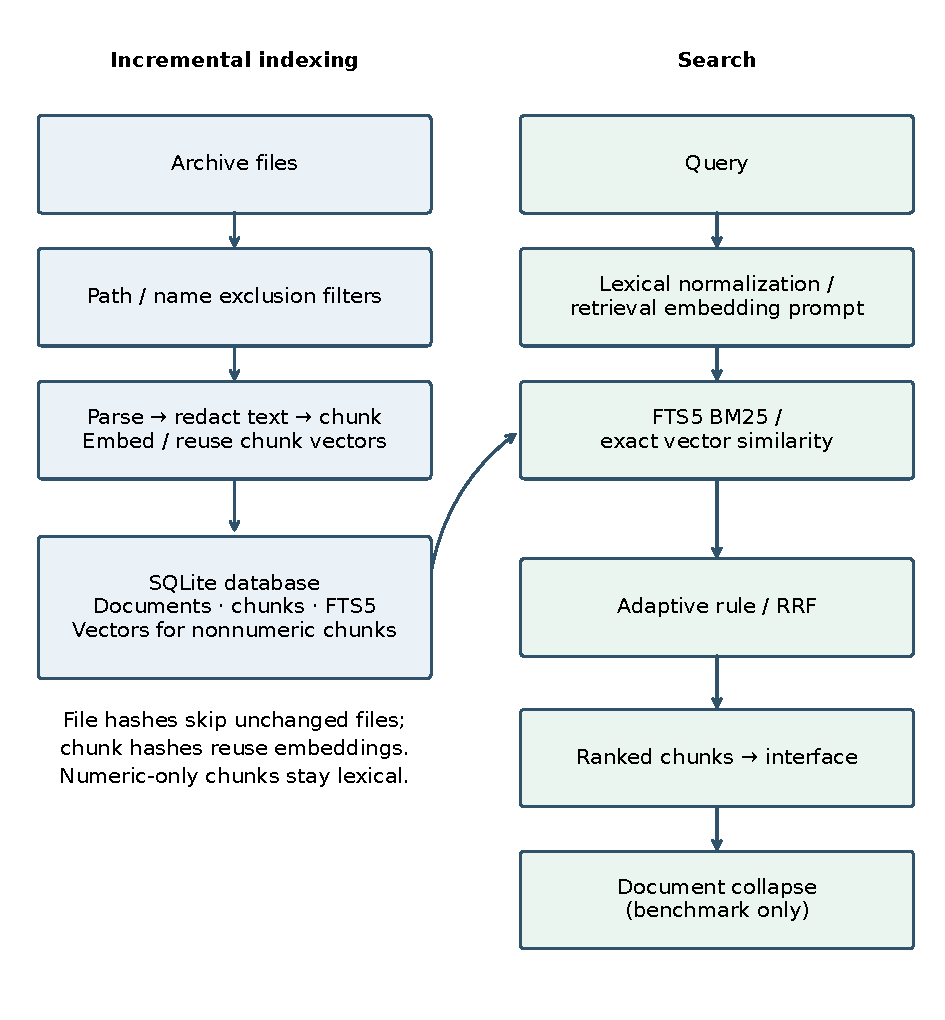
\includegraphics[width=\linewidth]{architecture.pdf}
\caption{Indexing and search data flow with the default local backend. Text redaction applies known patterns; images and audio are not content-redacted. Numeric-only chunks remain available to lexical search without vectors. Document collapse belongs to the benchmark, outside the query timer.}
\label{fig:architecture}
\end{figure}

\subsection{Lexical layer}
Words are runs of Unicode letters and digits that may be joined by a hyphen or an apostrophe, at least two characters long, lower-cased. The four apostrophe characters used in Ukrainian text (U+2019, U+02BC, U+2018 and the backtick) are mapped to the ASCII apostrophe before tokenization, so that \emph{м’ята} and \emph{мʼята} are one word. The FTS \code{terms} column stores every word followed by its normal forms from the pymorphy3 Ukrainian and Russian analyzers. A word containing a letter that exists only in Ukrainian (і, ї, є, ґ) goes through the Ukrainian analyzer only; other words go through both. When a dictionary knows the word, only dictionary normal forms are kept; the analyzers' guesses are used only for words that neither dictionary knows (Appendix~\ref{sec:intro-history} records the defect that this rule corrects).

Identifiers such as \code{36.101}, \code{19.6.0} or \code{RVZ0014A-2} (letter and digit runs joined by dots or slashes, or a hyphen followed by a digit) are matched as exact phrases, so a query for \code{36.109} never matches a document that contains only \code{36}. A query becomes an FTS5 expression in which each word is a disjunction of its surface and normal forms, the words are joined by OR, and an identifier clause, if present, is joined to the words by AND. Lexical ranking is FTS5 BM25.

\subsection{Dense layer}
The dense layer uses EmbeddingGemma~2 through SentenceTransformers, in bfloat16 on a GPU (the model card warns that float16 degrades the embeddings) and in float32 on a CPU. Documents are embedded as \code{title: <title> | text: <chunk>}; queries carry the model's retrieval prompt \code{task: search result | query:}, or \code{task: code retrieval | query:} when the code collection is searched. Vectors are L2-normalized; the 256-dimensional variant truncates them (Matryoshka truncation) and normalizes again. Pictures, PDF pages without a text layer and video frames (one every 5~s, at most 120 per video) are embedded as images in the same space. Sound is resampled to 16~kHz and embedded in 20~s windows with a 15~s step; when a transcript file accompanies a recording, the transcript lines that overlap a window become that window's text. A llama.cpp server running a GGUF build of the model is an optional text-only backend. Semantic search is exact: all vectors are held in memory and scored with one NumPy matrix--vector product, with no approximate nearest-neighbour index.

\subsection{Fusion}
Three ranking modes are available: lexical only, semantic only and hybrid. The default hybrid strategy (\sys{adaptive}) looks at the best lexical chunk. If it contains at least 90\% of the query words as whole words, the query is treated as a search for an exact phrase: only lexical results are returned, in BM25 order, except that chunks in which the query words occur in order within a slack of three words are moved to the front. Otherwise the semantic ranking comes first and the lexical results that it does not already contain follow; with no lexical match the result is purely semantic. Reciprocal-rank fusion with $k=60$ (\sys{rrf}) is the alternative hybrid strategy. In the interface, at most three chunks per document are shown, with a count of the remaining ones; benchmark runs collapse chunks to documents (Section~\ref{sec:method}).

\subsection{Incremental indexing}
A file is skipped when its size and modification time are unchanged, and also when its SHA-256 is unchanged; only then is it parsed again. Vectors are reused for chunks whose text hash is already stored, so editing a note re-embeds only the edited chunks. Files that disappeared are removed from their collection. Fragments of notes and documents with fewer than 20 letters (page numbers, punctuation) are dropped unless every fragment of the file is that short; pictures and sound are never dropped. Each run writes a report of indexed, skipped and failed files; a failure in one file does not stop the run.

\subsection{Privacy}
The default embedding backend processes document content locally. The optional llama.cpp client defaults to a loopback server; configuring an external \code{ARCHIVE\_LLAMA\_URL} sends text to that endpoint. Local processing therefore depends on the backend configuration. Directories \code{.ssh}, \code{.gnupg}, \code{.aws}, \code{.kube}, \code{.password-store}, \code{.docker} and key rings, and files whose names match key, certificate, password-store, environment and credential patterns (for example \code{*.pem}, \code{*.kdbx}, \code{id\_rsa*}, \code{.env}, \code{*secret*}, \code{*token*}) never enter the index. Inside indexed text, PEM private-key blocks, access keys in the formats of several common services (OpenAI, AWS, GitHub, Slack, bearer tokens) and explicit credential assignments such as \code{password=...} are replaced by a redaction marker before storage. The patterns cover known formats only; they are a safety net, not a guarantee. The redaction report counts kinds and never stores values.

% The UA-PAR benchmark. Counts from paper/results/corpus_summary.json and the manifest; query rules from paper/guidelines/queries.md.
\section{The UA-PAR benchmark}\label{sec:uapar}

\subsection{Sources and corpus}
\uapar{} imitates a researcher's archive with public-source material in Ukrainian and Russian (licences in Section~\ref{sec:availability}). The corpus has 7\,070 files in six parts. \emph{Notes}: 2\,945 Wikipedia articles (1\,960 Ukrainian, 985 Russian) on 25 topics, many of them technical, among them antennas, radio, LTE, software-defined radio, signal processing, microcontrollers, cryptography, machine learning, physics, history and literature; each article is stored as a Markdown note with its source line. \emph{Documents}: 400 further articles (260 Ukrainian, 140 Russian) rendered to 133 PDF, 134 DOCX and 133 PPTX files, so the archive has office formats. \emph{Tables}: 150 data.gov.ua datasets, 100 kept as CSV and 50 converted to XLSX. \emph{Code}: 1\,775 files from 30 Ukrainian-topic GitHub repositories, indexed as a code collection. \emph{Pictures}: 1\,000 Crossmodal-3600 images. \emph{Speech}: 800 FLEURS recordings, 400 Ukrainian and 400 Russian. The articles were collected by topic search with a page-and-resume collector; the SDR topic did not have enough long articles, so the notes are 55 short of the planned 3\,000 rather than padded with weakly related articles.

Not every collected file is indexable: archive-index skips generated and vendored files in repositories, so the full EG2 index holds 6\,054 documents (759 from the code part) and 96\,908 chunks. The text-only E5 index holds the 4\,137 text documents of the same corpus and no pictures or speech; Section~\ref{sec:results} shows that restricting EG2 to the same 4\,137 documents changes its nDCG@10 by $-0.0015$.

\subsection{Queries}
There are 200 queries in five categories with fixed quotas: 40 \emph{known-item} queries describing a specific document without quoting its title; 60 \emph{topical} queries that several documents may answer; 40 \emph{technical} queries containing identifiers, model numbers or standards as people write them; 30 \emph{cross-lingual} queries in Russian for a Ukrainian target or the reverse; and 30 \emph{no-answer} queries, plausible questions about things the corpus does not contain, often with invented model numbers. 126 queries are in Ukrainian and 74 in Russian. The 170 answerable queries were each written for one target note, which is recorded but is not the only relevant document. A validator checks the quotas and language shares, that every target exists, that no topical or cross-lingual query shares a run of more than five consecutive tokens with its target (no copying), and that every no-answer query has zero lexical matches in the index. All 200 queries pass.

The queries were written by GPT-6-Luna through the Codex CLI under these rules. Because the query writer must not grade its own queries, GPT grades never enter the relevance labels; they are used only to compare grading behaviour, which does not separate self-preference from general leniency (Section~\ref{sec:results}). The no-answer queries have no lexical match by construction, so BM25 returns nothing for them; the comparison of systems on these queries is therefore a check of whether a dense system ever abstains, not a fair contest between lexical and dense retrieval.

\subsection{Relevance assessments}
The assessment pool is the union of the first ten documents returned by each of the ten systems: 5\,572 query--document pairs for 200 queries. Separate shuffled sheets hide the retrieval system identities. Each judge sees the query, document title and beginning, limited to 1\,200 characters; speech records include the source transcript. Grades are 0 (unrelated), 1 (partly relevant) and 2 (directly answers the query). These labels describe the visible snippet rather than an inspection of the complete document.

The initial primary judge is Gemini~3.8 Flash, invoked through \code{agy} in batches of 50. Gemma~4 12B through Ollama provides the main sensitivity assessment, and Gemma~4 E4B provides an ancillary open-weights assessment. GPT-6-Luna authored the queries; its grades are reported only for comparison and never enter the primary or sensitivity relevance labels. All initial sheets are preserved. Gemini and Gemma share a provider, so separate grading does not establish independence of training data or errors.

Initial Gemini and Gemma~4 12B disagree on 1\,091 pairs. For the reviewed variant, a separate Gemini pass reassesses those pairs with both initial grades visible under neutral A/B labels, balanced in presentation order. Agreed grades are retained. This is a within-model review, not independent third-judge adjudication. Retrieval results are compared across initial Gemini, initial Gemma~4 12B and reviewed Gemini. The choice of the primary judge followed inspection of agreement and target/no-answer diagnostics and preceded the reported aggregate effectiveness comparison of systems; it was not preregistered. No completed human relevance audit is claimed.

All 170 answerable query targets are notes, and 134 targets occur in the depth-10 pool. Consequently, target-grade diagnostics use a denominator of 134 and do not measure accuracy on the complete target set. The 30 designated no-answer queries are analysed separately.

\subsection{Multimodal subsets}
Text-to-image and text-to-speech retrieval are evaluated outside the pooled benchmark, using caption--image and transcript--recording pairings from the source datasets rather than separately collected relevance judgements. For pictures, the query is the first Ukrainian or Russian Crossmodal-3600 caption of an image, and the gold item is that image among all 1\,000. For speech, the query is the FLEURS transcript of a sentence and the gold items are the recordings of that sentence; FLEURS is n-way parallel, so a Russian transcript can query Ukrainian recordings of the same sentence and the reverse. Each condition is scored three ways: against the audio vector of a recording, against its transcript embedded as text, and against the better of the two. When the query is the transcript of the recording itself, the text and combined scores are an upper bound, not a retrieval result; the audio-only and cross-lingual conditions carry the claims.

% Evaluation methodology. Resource protocol as implemented in paper/eval/run_efficiency.py and ann_scaling.py.
\section{Evaluation methodology}\label{sec:method}

\subsection{Systems and units}
All systems use the same archive-index search implementation with explicit configuration switches. The comparison includes plain and lemmatized BM25, full-dimensional EmbeddingGemma~2, a 256-dimensional EG2 variant, multilingual-E5, reciprocal-rank fusion, the adaptive system and three ablations removing phrase reranking, identifier handling or short-fragment filtering. Runs are document-level: the first retrieved chunk determines each document's rank, and subsequent chunks of that document are collapsed. Up to 100 documents are retained per query. The E5 index is text-only, unlike the full EG2 indexes; the differing candidate universes are reported as a limitation.

\subsection{Query population and metrics}
Retrieval means use the same 170 answerable queries for every system and judge variant, with each query weighted equally. The 30 designated no-answer queries are retained in the relevance files but excluded from those means; empty retrieval and positive-labelled results on them are reported separately. An answerable query with no positive pooled judgement remains in the average with score zero.

The primary metric is nDCG@10, using linear relevance gains 0, 1 and 2, discounted by $\log_2(i+1)$ at rank $i$ and normalized by the ideal ranking of the judged documents. Secondary metrics are reciprocal rank at 10, success at 1 and 5, and recall at 100. Binary metrics treat grades 1 and 2 as relevant. Every system's retrieved top-10 documents are judged, but judgements outside the depth-10 union are incomplete. Recall at 100 is therefore relative to the known relevant pool, not exhaustive corpus recall. Results are also grouped by query category and language.

\subsection{Uncertainty and comparisons}
Confidence intervals for query means and paired mean differences use a percentile bootstrap over queries with 10\,000 resamples and seed 2026. Two-sided paired sign-flip randomization tests use 10\,000 resamples and the add-one correction $(b+1)/(10\,000+1)$. Each metric and judge variant has a family of nine comparisons against the full adaptive system; p-values receive Holm adjustment within that family, with threshold 0.05. The original morphology research question is additionally assessed by a separately labelled paired lemma-versus-plain BM25 contrast on nDCG@10; its unadjusted p-value is not part of the adaptive comparison family. Neither separate confidence-interval overlap nor failure to reject a difference is interpreted as equivalence.

The initial inter-judge agreement report uses linear-weighted Cohen's kappa with a 95\% interval from 2\,000 query-level bootstrap resamples. Resampling queries, rather than individual judgement pairs, preserves within-query clustering. These agreement intervals are separate from the 10\,000-resample retrieval intervals. Rankings and pairwise ordering changes are reported for each relevance variant; numerically equal means within $10^{-12}$ share a rank.

\subsection{Reproducibility and evidence}
Initial judgement sheets, query definitions, corpus manifest, retrieval runs and available call logs are frozen before the reported aggregate effectiveness comparison is computed. A SHA-256 manifest validates those inputs; a separate prepared-review record binds the review to its original disagreements and presentation order. Structured call responses are logged with model, conversation and usage metadata when available. Canonical labels replace only disagreement grades after complete review, preserving every agreed grade. Report tables and figures are generated from the resulting JSON artifacts rather than maintained as independent numerical copies.

Unit and integration checks establish implementation behaviour; the public benchmark provides model-labelled retrieval evidence; the separate multimodal experiments use source-dataset labels. These evidence types do not substitute for a human relevance audit or deployment measurements.

\subsection{Resource measurements}
Query latency is the wall time of query embedding and chunk search in the evaluation harness, including lexical and semantic retrieval and fusion with a candidate limit of 400 chunks. The timer stops before document collapse and path resolution; these measurements are not end-to-end interface latency. Each system answers all 200 queries once as a warm-up and then once more under measurement, in one process, first with the GPU visible and then with \code{CUDA\_VISIBLE\_DEVICES} empty (the embedding models then run on the CPU in float32). During each measured pass the harness records per-core CPU use from \code{/proc/stat}, CPU seconds per thread of the process from \code{/proc/self/task}, the change in interrupt counts per core from \code{/proc/interrupts}, the peak resident set size, and GPU memory sampled every 0.2~s with \code{nvidia-smi}. The machine was an ordinary desktop session; the one-minute load average before each step is written to the measurement log.

Indexing cost is measured on a fixed random sample of the corpus (seed 2026: 300 notes, 40 documents, 15 tables, 60 pictures and 60 recordings) indexed by the \code{archive} command into an empty database with the GPU. The CPU run uses a fifth-sized sample: 60 notes, 8 documents, 3 tables, 12 pictures and 12 recordings. The two samples differ in size and composition, so their wall times do not estimate a paired CPU/GPU speedup. The sizes of the four full benchmark indexes are reported as built.

For quantization, the text chunks of the full index (84\,788 vectorized rows in text collections) are embedded again by GGUF builds of EmbeddingGemma~2 (f16, Q8\_0, Q4\_K\_M) served by llama.cpp with mean pooling, with the same \code{title: \ldots{} | text: \ldots} prefixes; queries use the same retrieval prompt. Dense retrieval with each build runs on the 4\,137 text documents and is compared with the SentenceTransformers bfloat16 model on the same documents (\sys{dense\_eg2\_text}) under the same labels. Documents that a quantized run brings into its top~10 but that no judge saw are counted as non-relevant, and their share is reported. The text collections include 21 PDF-page rows embedded as images by the full model. GGUF instead encodes their stored text (485 characters in total); 84\,767 rows are text inputs. Thus identical document candidates do not mean identical input modality for every chunk, and the comparison does not isolate quantization alone.

Scaling of exact dense search is measured outside archive-index with collections grown from the 86\,726 real EG2 vectors to $10^5$, $3\cdot10^5$, $10^6$ and $2\cdot10^6$ vectors; the added vectors are noisy copies of real ones (Gaussian noise, $\sigma=0.05$, renormalized), so the collections are synthetic. Each of the 200 UA-PAR query vectors is searched one at a time with an optimized exact NumPy top-10 selection (matrix product and \code{argpartition}), an exact Faiss index and an HNSW index ($M=32$, construction depth 200, search depth 64 and 256). A sequential follow-up calls the actual archive-index vector-ranking method on the same matrices: candidate gathering, full \code{argsort} and construction of 400 result tuples, excluding the SQLite cache-version poll. This distinguishes the optimized reference from the deployed algorithm. HNSW recall@10 counts matching vector IDs against the NumPy reference; ties and floating-point differences are not credited as equivalent IDs. Agreement between the exact Faiss and NumPy rankings is audited separately, together with the fraction of Faiss results at or above the reference tenth score within $10^{-6}$.

\subsection{Software and hardware}
All measurements ran on one laptop: Intel Core i9-14900HX (32 logical CPUs), 31~GiB RAM, NVIDIA GeForce RTX 4060 Laptop GPU with 8~GB, Linux 7.0. Software: Python 3.13.14, PyTorch 2.14.1, Transformers 5.19.0, SentenceTransformers 6.1.0, NumPy 2.5.4, SQLite 3.53.1, pymorphy3 2.0.6, ir-measures 0.4.3, llama.cpp commit \code{8bb3cf0}, and Faiss 1.15.1 in a separate environment for the scaling experiment. The full list is stored in \code{efficiency.json}.

% Source-backed tables/figures; final comparison interpretation is inserted after review.
\section{Results}\label{sec:results}
% Generated from primary=gemini_reviewed; see ../manifest.json for source SHA-256.
\newif\ifpaperlatency
\paperlatencytrue
\newif\ifpaperindexing
\paperindexingtrue
\newif\ifpapergguf
\papergguftrue
\newif\ifpaperann
\paperanntrue
\newif\ifpaperfield
\paperfieldtrue
\newif\ifpaperextension
\paperextensiontrue
\newif\ifpaperextensionunique
\paperextensionuniquetrue


\subsection{Retrieval and judge sensitivity}
Table~\ref{tab:retrieval} reports all ten systems on the same answerable-query population. Confidence intervals describe query-level variation under the reported labels; they do not capture uncertainty in the labels themselves. Table~\ref{tab:judge-sensitivity} and Figure~\ref{fig:judge-sensitivity} preserve the initial and reviewed variants. Gemini review is within-model, and Gemini and Gemma share a provider.

E5 has the highest mean nDCG@10 under all three principal relevance variants. Its lead over adaptive does not reach the 0.05 threshold after Holm correction in any variant; this does not establish equivalence. Adaptive outperforms both BM25 baselines on the primary endpoint after correction, but shows no statistically detectable advantage over EG2 alone or RRF. Removing phrase reranking leaves the evaluated scores unchanged; the other adaptive ablation differences in nDCG@10 are small and not statistically detectable on this query set. These findings do not support a general claim that adaptive fusion improves over dense retrieval.

Lemmatization improves mean BM25 nDCG@10 under all three variants. The separately reported paired morphology contrast supports the difference under initial and reviewed Gemini labels, while its interval crosses zero under Gemma~4 12B labels. Thus the strength of the morphology finding depends on relevance assessment. The within-model review changes 334 of the 5\,572 initial Gemini labels; all 4\,481 initially agreed pairs remain unchanged.

\begin{table}[p]
\centering
\caption{Document retrieval on 170 answerable queries. Means and 95\% query-bootstrap intervals use Gemini labels after the within-model disagreement review. The two panels preserve all five metrics. A dagger marks a paired difference from adaptive at Holm-adjusted $p<0.05$, not necessarily an improvement. R@100 is pool-relative. E5 uses a smaller text-only candidate universe.}
\label{tab:retrieval}
% Generated from primary=gemini_reviewed; see ../manifest.json for source SHA-256.
% Means with 95% bootstrap CI; n=170. R@100 is pool-relative under incomplete judgments. Significance: paired comparison against adaptive only, \(p_{\mathrm{Holm}}<0.05\).
\begingroup\small\setlength{\tabcolsep}{4pt}\renewcommand{\arraystretch}{1.3}
\noindent\begin{tabularx}{\linewidth}{@{}l*{3}{>{\centering\arraybackslash}X}@{}}
\toprule
System & nDCG@10 & R@100\textsuperscript{pool} & RR@10 \\
\midrule
bm25\_plain & \shortstack{0.450\textsuperscript{\textdagger} \\ {\footnotesize[0.413, 0.487]}} & \shortstack{0.648\textsuperscript{\textdagger} \\ {\footnotesize[0.611, 0.685]}} & \shortstack{0.738\textsuperscript{\textdagger} \\ {\footnotesize[0.682, 0.790]}} \\
bm25\_lemma & \shortstack{0.482\textsuperscript{\textdagger} \\ {\footnotesize[0.446, 0.518]}} & \shortstack{0.724\textsuperscript{\textdagger} \\ {\footnotesize[0.693, 0.755]}} & \shortstack{0.753\textsuperscript{\textdagger} \\ {\footnotesize[0.701, 0.802]}} \\
dense\_eg2 & \shortstack{0.633 \\ {\footnotesize[0.601, 0.664]}} & \shortstack{0.911 \\ {\footnotesize[0.890, 0.930]}} & \shortstack{0.872 \\ {\footnotesize[0.832, 0.910]}} \\
dense\_e5 & \shortstack{0.674 \\ {\footnotesize[0.647, 0.700]}} & \shortstack{0.880 \\ {\footnotesize[0.853, 0.906]}} & \shortstack{0.927 \\ {\footnotesize[0.894, 0.956]}} \\
rrf & \shortstack{0.630 \\ {\footnotesize[0.601, 0.660]}} & \shortstack{0.960\textsuperscript{\textdagger} \\ {\footnotesize[0.946, 0.972]}} & \shortstack{0.873 \\ {\footnotesize[0.835, 0.910]}} \\
adaptive & \shortstack{0.629 \\ {\footnotesize[0.596, 0.660]}} & \shortstack{0.908 \\ {\footnotesize[0.887, 0.928]}} & \shortstack{0.866 \\ {\footnotesize[0.826, 0.905]}} \\
adaptive-phrase & \shortstack{0.629 \\ {\footnotesize[0.596, 0.660]}} & \shortstack{0.908 \\ {\footnotesize[0.887, 0.928]}} & \shortstack{0.866 \\ {\footnotesize[0.826, 0.905]}} \\
adaptive-ident & \shortstack{0.629 \\ {\footnotesize[0.597, 0.661]}} & \shortstack{0.912 \\ {\footnotesize[0.892, 0.931]}} & \shortstack{0.866 \\ {\footnotesize[0.826, 0.905]}} \\
adaptive-short & \shortstack{0.629 \\ {\footnotesize[0.597, 0.660]}} & \shortstack{0.908 \\ {\footnotesize[0.887, 0.928]}} & \shortstack{0.866 \\ {\footnotesize[0.826, 0.905]}} \\
dense\_eg2\_256 & \shortstack{0.611 \\ {\footnotesize[0.577, 0.643]}} & \shortstack{0.888\textsuperscript{\textdagger} \\ {\footnotesize[0.863, 0.911]}} & \shortstack{0.873 \\ {\footnotesize[0.830, 0.913]}} \\
\bottomrule
\end{tabularx}\endgroup

\par\medskip
% Means with 95% bootstrap CI; n=170. R@100 is pool-relative under incomplete judgments. Significance: paired comparison against adaptive only, \(p_{\mathrm{Holm}}<0.05\).
\begingroup\small\setlength{\tabcolsep}{4pt}\renewcommand{\arraystretch}{1.3}
\noindent\begin{tabularx}{\linewidth}{@{}l*{2}{>{\centering\arraybackslash}X}@{}}
\toprule
System & Success@1 & Success@5 \\
\midrule
bm25\_plain & \shortstack{0.635\textsuperscript{\textdagger} \\ {\footnotesize[0.559, 0.706]}} & \shortstack{0.876\textsuperscript{\textdagger} \\ {\footnotesize[0.824, 0.924]}} \\
bm25\_lemma & \shortstack{0.624\textsuperscript{\textdagger} \\ {\footnotesize[0.547, 0.694]}} & \shortstack{0.929 \\ {\footnotesize[0.888, 0.965]}} \\
dense\_eg2 & \shortstack{0.794 \\ {\footnotesize[0.729, 0.853]}} & \shortstack{0.971 \\ {\footnotesize[0.941, 0.994]}} \\
dense\_e5 & \shortstack{0.876 \\ {\footnotesize[0.824, 0.924]}} & \shortstack{0.988 \\ {\footnotesize[0.971, 1.000]}} \\
rrf & \shortstack{0.788 \\ {\footnotesize[0.724, 0.847]}} & \shortstack{0.976 \\ {\footnotesize[0.953, 0.994]}} \\
adaptive & \shortstack{0.782 \\ {\footnotesize[0.718, 0.841]}} & \shortstack{0.971 \\ {\footnotesize[0.941, 0.994]}} \\
adaptive-phrase & \shortstack{0.782 \\ {\footnotesize[0.718, 0.841]}} & \shortstack{0.971 \\ {\footnotesize[0.941, 0.994]}} \\
adaptive-ident & \shortstack{0.782 \\ {\footnotesize[0.718, 0.841]}} & \shortstack{0.971 \\ {\footnotesize[0.941, 0.994]}} \\
adaptive-short & \shortstack{0.782 \\ {\footnotesize[0.718, 0.841]}} & \shortstack{0.971 \\ {\footnotesize[0.941, 0.994]}} \\
dense\_eg2\_256 & \shortstack{0.818 \\ {\footnotesize[0.759, 0.871]}} & \shortstack{0.953 \\ {\footnotesize[0.918, 0.982]}} \\
\bottomrule
\end{tabularx}\endgroup

\par\smallskip
{\footnotesize \textdagger: p\textsubscript{Holm}<0.05, adaptive; R@100: pool-relative.}

\end{table}

\begin{table}[p]
\centering
\caption{Sensitivity of nDCG@10 to relevance assessment. Initial Gemini and Gemma~4 12B grades are retained; the reviewed variant changes only their disagreements. The same frozen runs and 170 queries are used throughout. GPT grades do not enter this comparison.}
\label{tab:judge-sensitivity}
% Generated from primary=gemini_reviewed; see ../manifest.json for source SHA-256.
% nDCG@10 with 95% bootstrap CI. Gemini reviewed is a within-model review. Gemini/Gemma12 share a provider family. No GPT or E4B in this principal comparison.
\begingroup\small\setlength{\tabcolsep}{4pt}\renewcommand{\arraystretch}{1.3}
\noindent\begin{tabularx}{\linewidth}{@{}l*{3}{>{\centering\arraybackslash}X}@{}}
\toprule
System & Gemini initial & Gemma12 initial & Gemini reviewed \\
\midrule
bm25\_plain & \shortstack{0.453 \\ {\footnotesize[0.416, 0.491]}} & \shortstack{0.500 \\ {\footnotesize[0.462, 0.536]}} & \shortstack{0.450 \\ {\footnotesize[0.413, 0.487]}} \\
bm25\_lemma & \shortstack{0.489 \\ {\footnotesize[0.453, 0.526]}} & \shortstack{0.519 \\ {\footnotesize[0.482, 0.554]}} & \shortstack{0.482 \\ {\footnotesize[0.446, 0.518]}} \\
dense\_eg2 & \shortstack{0.644 \\ {\footnotesize[0.613, 0.674]}} & \shortstack{0.681 \\ {\footnotesize[0.652, 0.709]}} & \shortstack{0.633 \\ {\footnotesize[0.601, 0.664]}} \\
dense\_e5 & \shortstack{0.685 \\ {\footnotesize[0.657, 0.711]}} & \shortstack{0.698 \\ {\footnotesize[0.671, 0.725]}} & \shortstack{0.674 \\ {\footnotesize[0.647, 0.700]}} \\
rrf & \shortstack{0.641 \\ {\footnotesize[0.612, 0.669]}} & \shortstack{0.665 \\ {\footnotesize[0.636, 0.694]}} & \shortstack{0.630 \\ {\footnotesize[0.601, 0.660]}} \\
adaptive & \shortstack{0.639 \\ {\footnotesize[0.608, 0.669]}} & \shortstack{0.675 \\ {\footnotesize[0.647, 0.703]}} & \shortstack{0.629 \\ {\footnotesize[0.596, 0.660]}} \\
adaptive-phrase & \shortstack{0.639 \\ {\footnotesize[0.608, 0.669]}} & \shortstack{0.675 \\ {\footnotesize[0.647, 0.703]}} & \shortstack{0.629 \\ {\footnotesize[0.596, 0.660]}} \\
adaptive-ident & \shortstack{0.639 \\ {\footnotesize[0.608, 0.669]}} & \shortstack{0.676 \\ {\footnotesize[0.648, 0.704]}} & \shortstack{0.629 \\ {\footnotesize[0.597, 0.661]}} \\
adaptive-short & \shortstack{0.639 \\ {\footnotesize[0.608, 0.669]}} & \shortstack{0.675 \\ {\footnotesize[0.647, 0.703]}} & \shortstack{0.629 \\ {\footnotesize[0.597, 0.660]}} \\
dense\_eg2\_256 & \shortstack{0.622 \\ {\footnotesize[0.589, 0.654]}} & \shortstack{0.665 \\ {\footnotesize[0.633, 0.696]}} & \shortstack{0.611 \\ {\footnotesize[0.577, 0.643]}} \\
\bottomrule
\end{tabularx}\endgroup

\end{table}

\begin{figure}[p]
\centering
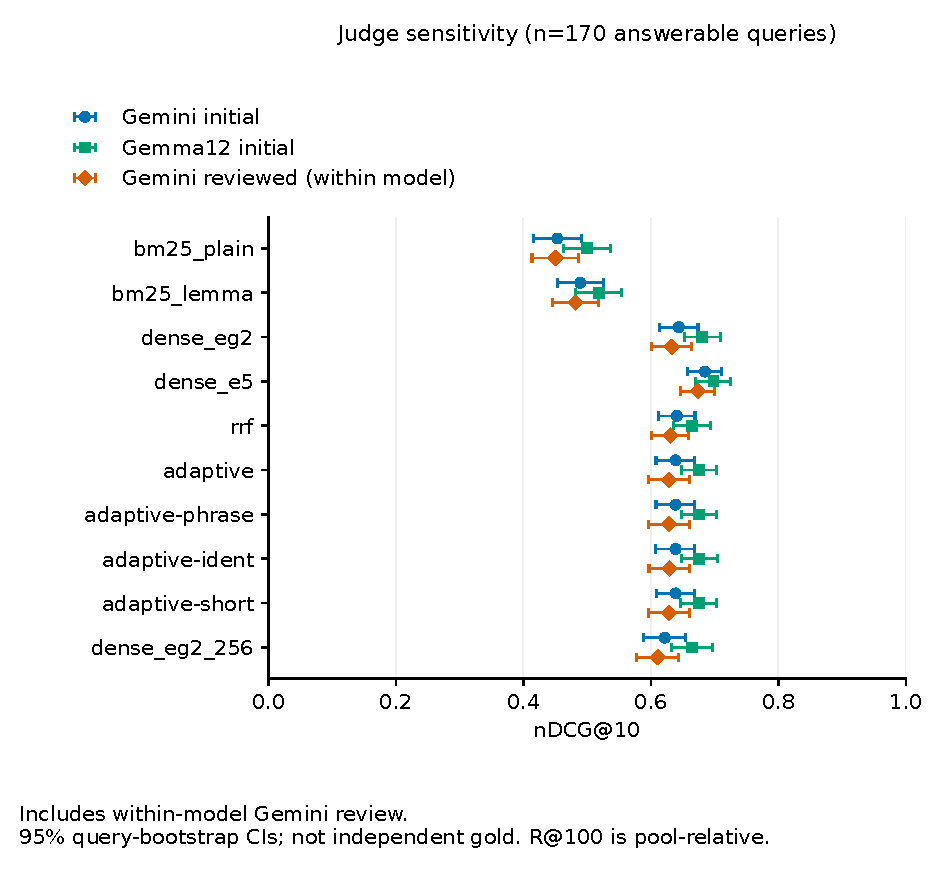
\includegraphics[width=\linewidth]{judge_sensitivity.pdf}
\caption{System scores and 95\% query-bootstrap intervals across relevance variants. Differences between separate intervals do not replace paired statistical comparisons.}
\label{fig:judge-sensitivity}
\end{figure}

\begin{figure}[p]
\centering
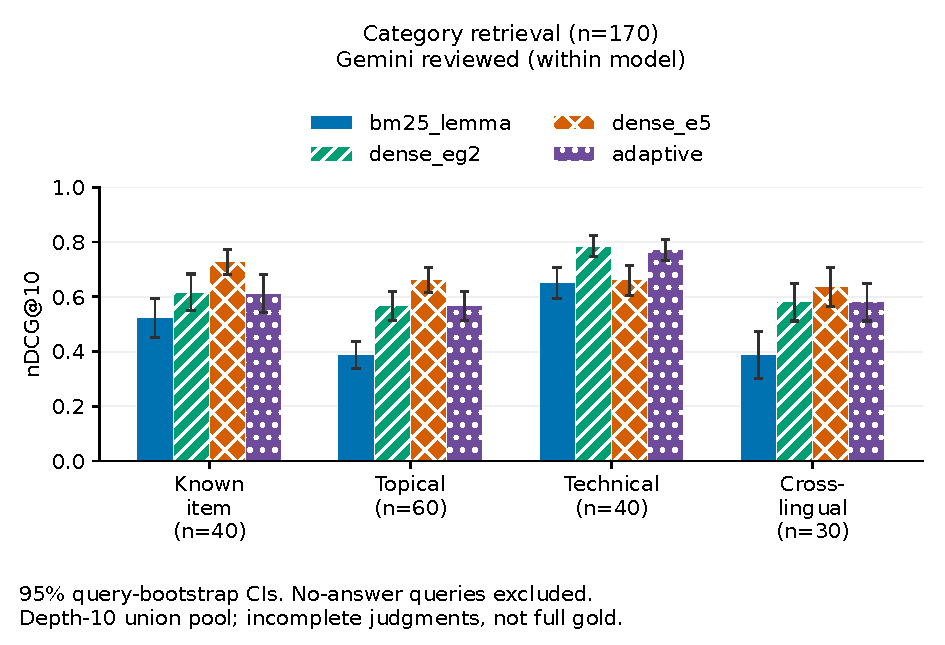
\includegraphics[width=\linewidth]{category_ndcg.pdf}
\caption{nDCG@10 by query category for four principal systems under the primary relevance variant. Each category uses its own query-bootstrap interval. No-answer queries are excluded.}
\label{fig:categories}
\end{figure}

\subsection{Controls}
\paragraph{Candidate universe.} E5 searches 4\,137 text documents; the full EG2 index holds 6\,054 documents, including media. Restricting EG2 to the same 4\,137 text documents (\sys{dense\_eg2\_text}) changes its nDCG@10 by $-0.0015$ under reviewed Gemini labels (0.633 to 0.631); 0.29\% of its top-10 documents were not in the judged pool. The paired difference EG2$_{\mathrm{text}}-{}$E5 is $-0.042$ nDCG@10 (95\% CI $-0.078$ to $-0.006$, unadjusted $p=0.018$) with reviewed Gemini labels and $-0.019$ ($-0.052$ to $0.014$, $p=0.26$) with Gemma~4 12B labels (Table~\ref{tab:encoder-control}). Thus the candidate restriction has a small point effect in this control, while statistical support for the encoder difference depends on the labels. These exploratory comparisons use unadjusted p-values and an incomplete judgement pool.

\begin{table}[p]
\centering
\caption{E5 against EG2 on the same 4\,137 text documents. $\Delta$ is the paired difference from E5 with a 95\% query-bootstrap interval and an unadjusted sign-flip $p$; unjudged documents count as non-relevant, and their share is shown.}
\label{tab:encoder-control}
% Generated from primary=gemini_reviewed; see ../manifest.json for source SHA-256.
\noindent\textbf{Gemini reviewed}
\par\smallskip
% E5 against EG2 on the same 4137 text documents; source encoder_control.json
\begingroup\small\setlength{\tabcolsep}{4pt}\renewcommand{\arraystretch}{1.3}
\noindent\begin{tabularx}{\linewidth}{@{}l*{4}{>{\centering\arraybackslash}X}@{}}
\toprule
System & nDCG@10 & $\Delta$ [95\% CI] vs E5 & p & Unjudged@10 \\
\midrule
\sys{dense\_e5} & 0.674 & -- & -- & 0.000 \\
\sys{dense\_eg2} & 0.633 & \shortstack{-0.041 \\ {\footnotesize[-0.077, -0.005]}} & 0.023 & 0.000 \\
\sys{dense\_eg2\_text} & 0.631 & \shortstack{-0.042 \\ {\footnotesize[-0.078, -0.006]}} & 0.018 & 0.003 \\
\bottomrule
\end{tabularx}\endgroup

\par\medskip
\noindent\textbf{Gemini initial}
\par\smallskip
% E5 against EG2 on the same 4137 text documents; source encoder_control.json
\begingroup\small\setlength{\tabcolsep}{4pt}\renewcommand{\arraystretch}{1.3}
\noindent\begin{tabularx}{\linewidth}{@{}l*{4}{>{\centering\arraybackslash}X}@{}}
\toprule
System & nDCG@10 & $\Delta$ [95\% CI] vs E5 & p & Unjudged@10 \\
\midrule
\sys{dense\_e5} & 0.685 & -- & -- & 0.000 \\
\sys{dense\_eg2} & 0.644 & \shortstack{-0.041 \\ {\footnotesize[-0.075, -0.007]}} & 0.020 & 0.000 \\
\sys{dense\_eg2\_text} & 0.642 & \shortstack{-0.042 \\ {\footnotesize[-0.077, -0.009]}} & 0.014 & 0.003 \\
\bottomrule
\end{tabularx}\endgroup

\par\medskip
\noindent\textbf{Gemma 12B initial}
\par\smallskip
% E5 against EG2 on the same 4137 text documents; source encoder_control.json
\begingroup\small\setlength{\tabcolsep}{4pt}\renewcommand{\arraystretch}{1.3}
\noindent\begin{tabularx}{\linewidth}{@{}l*{4}{>{\centering\arraybackslash}X}@{}}
\toprule
System & nDCG@10 & $\Delta$ [95\% CI] vs E5 & p & Unjudged@10 \\
\midrule
\sys{dense\_e5} & 0.698 & -- & -- & 0.000 \\
\sys{dense\_eg2} & 0.681 & \shortstack{-0.018 \\ {\footnotesize[-0.050, +0.015]}} & 0.285 & 0.000 \\
\sys{dense\_eg2\_text} & 0.680 & \shortstack{-0.019 \\ {\footnotesize[-0.052, +0.014]}} & 0.258 & 0.003 \\
\bottomrule
\end{tabularx}\endgroup

\end{table}

\paragraph{Whole-word coverage.} The adaptive rule's exact-phrase test counted substrings (Appendix~\ref{sec:intro-history}). With the corrected rule, the top~10 changes for one query of 200 in each adaptive variant, and adaptive nDCG@10 moves from 0.629 to 0.627 (reviewed Gemini), 0.639 to 0.637 (initial Gemini) and stays at 0.675 (Gemma~4 12B). The frozen primary results are retained; the corrected point score does not create an adaptive advantage over dense EG2.

\subsection{Judges}
Table~\ref{tab:judge-checks} reports grades over the whole pool and on two construction-based diagnostic subsets: pooled authored targets and designated no-answer pairs. These expectations are not independent human labels. Table~\ref{tab:judge-agreement} reports pairwise agreement. Gemini, the two Gemma models and GPT-6-Luna agree with linear-weighted $\kappa$ between 0.535 and 0.652. Gemini gives the target document of a known-item or other answerable query grade~2 in 85.8\% of the 134 pooled targets, Gemma~4 12B in 67.2\%: the larger Gemma model agrees best with Gemini overall but rarely gives full marks. On the 708 pooled pairs of no-answer queries, Gemini, Gemma~4 12B and Gemma~4 E4B give grade~0 in 90.4\%, 91.2\% and 93.5\% of pairs.

GPT-6-Luna, which wrote the queries, is the most lenient judge: its mean grade is 0.633 against 0.421--0.447 for the other judges, and it gives a positive grade to 24.3\% of the no-answer pairs, against 6.5--9.6\% for the others. Its grades are higher than every other judge's on average by 0.19--0.21. This is consistent with self-preference by the query author, but general leniency would produce the same pattern. The present comparison cannot distinguish those explanations. GPT grades are not used in any relevance label.

\begin{table}[p]
\centering
\caption{Judges on the 5\,572 pooled pairs: mean grade, grade counts, and construction-based checks (share of pooled answerable-query targets graded 2; share of pooled no-answer pairs graded 0).}
\label{tab:judge-checks}
% Generated from primary=gemini_reviewed; see ../manifest.json for source SHA-256.
% grades on the whole pool and known-answer checks; source judges.json
\begingroup\small\setlength{\tabcolsep}{4pt}\renewcommand{\arraystretch}{1.3}
\noindent\begin{tabularx}{\linewidth}{@{}l*{5}{>{\centering\arraybackslash}X}@{}}
\toprule
Judge & Pairs & Mean grade & 0 / 1 / 2 & Target = 2, \% & No-answer = 0, \% \\
\midrule
Gemini 3.8 Flash & 5\,572 & 0.421 & 3\,522 / 1\,756 / 294 & 85.8 (n=134) & 90.4 (n=708) \\
Gemma 4 12B & 5\,572 & 0.447 & 3\,316 / 2\,024 / 232 & 67.2 (n=134) & 91.2 (n=708) \\
Gemma 4 E4B & 5\,572 & 0.438 & 3\,519 / 1\,665 / 388 & 74.6 (n=134) & 93.5 (n=708) \\
GPT-6-Luna & 5\,572 & 0.633 & 2\,554 / 2\,510 / 508 & 91.8 (n=134) & 75.7 (n=708) \\
\bottomrule
\end{tabularx}\endgroup

\end{table}

\begin{table}[p]
\centering
\caption{Pairwise agreement between judges on the same 5\,572 pairs: linear-weighted Cohen's $\kappa$ with a 95\% interval from 2\,000 query-level bootstrap resamples, exact agreement, and the mean grade difference.}
\label{tab:judge-agreement}
% Generated from primary=gemini_reviewed; see ../manifest.json for source SHA-256.
% linear-weighted kappa, CI by resampling queries; source judges.json
\begingroup\small\setlength{\tabcolsep}{4pt}\renewcommand{\arraystretch}{1.3}
\noindent\begin{tabularx}{\linewidth}{@{}l*{4}{>{\centering\arraybackslash}X}@{}}
\toprule
Judges & Pairs & Weighted $\kappa$ [95\% CI] & Exact agreement & Mean A$-$B \\
\midrule
Gemini 3.8 Flash – Gemma 4 12B & 5\,572 & 0.652 [0.625, 0.677] & 0.804 & -0.026 \\
Gemini 3.8 Flash – Gemma 4 E4B & 5\,572 & 0.591 [0.559, 0.622] & 0.768 & -0.017 \\
Gemini 3.8 Flash – GPT-6-Luna & 5\,572 & 0.621 [0.595, 0.644] & 0.759 & -0.212 \\
Gemma 4 12B – Gemma 4 E4B & 5\,572 & 0.650 [0.625, 0.674] & 0.799 & +0.008 \\
Gemma 4 12B – GPT-6-Luna & 5\,572 & 0.586 [0.559, 0.612] & 0.741 & -0.186 \\
Gemma 4 E4B – GPT-6-Luna & 5\,572 & 0.535 [0.506, 0.564] & 0.700 & -0.195 \\
\bottomrule
\end{tabularx}\endgroup

\end{table}

\subsection{Images and speech}
Table~\ref{tab:multimodal} reports separate image-caption and speech-transcript retrieval tasks. These point estimates have no computed confidence intervals. The monolingual text-only speech condition uses the same transcript as query and indexed text, so it is a ceiling condition rather than a realistic paraphrased-query evaluation. Cross-language queries are parallel source transcripts and also do not represent arbitrary conversational audio search.

\begin{table}[p]
\centering
\caption{Separate source-labelled multimodal tasks: query and candidate counts, followed by point estimates. No confidence intervals are fabricated. Speech text mode indexes the transcript; both mode combines transcript and audio.}
\label{tab:multimodal}
% Generated from primary=gemini_reviewed; see ../manifest.json for source SHA-256.
% Separate multimodal tasks; confidence intervals unavailable in source (not fabricated).
\begingroup\small\setlength{\tabcolsep}{4pt}\renewcommand{\arraystretch}{1.3}
\noindent\begin{tabularx}{\linewidth}{@{}l*{2}{>{\centering\arraybackslash}X}@{}}
\toprule
Mode & Queries & Items \\
\midrule
Image / ru & 1000 & 1000 \\
Image / uk & 1000 & 1000 \\
Speech / ru->ru / audio & 265 & 400 \\
Speech / ru->ru / both & 265 & 400 \\
Speech / ru->ru / text & 265 & 400 \\
Speech / ru->uk / audio & 194 & 400 \\
Speech / ru->uk / both & 194 & 400 \\
Speech / ru->uk / text & 194 & 400 \\
Speech / uk->ru / audio & 194 & 400 \\
Speech / uk->ru / both & 194 & 400 \\
Speech / uk->ru / text & 194 & 400 \\
Speech / uk->uk / audio & 262 & 400 \\
Speech / uk->uk / both & 262 & 400 \\
Speech / uk->uk / text & 262 & 400 \\
\bottomrule
\end{tabularx}\endgroup

\par\medskip
% Point estimates only; confidence intervals unavailable. Recall is task-specific.
\begingroup\small\setlength{\tabcolsep}{4pt}\renewcommand{\arraystretch}{1.3}
\noindent\begin{tabularx}{\linewidth}{@{}l*{4}{>{\centering\arraybackslash}X}@{}}
\toprule
Mode & recall@1 & recall@5 & recall@10 & mrr \\
\midrule
Image / ru & 0.889 & 0.983 & 0.994 & 0.932 \\
Image / uk & 0.857 & 0.977 & 0.986 & 0.909 \\
Speech / ru->ru / audio & 0.996 & 1.000 & 1.000 & 0.997 \\
Speech / ru->ru / both & 1.000 & 1.000 & 1.000 & 1.000 \\
Speech / ru->ru / text & 1.000 & 1.000 & 1.000 & 1.000 \\
Speech / ru->uk / audio & 0.985 & 1.000 & 1.000 & 0.991 \\
Speech / ru->uk / both & 1.000 & 1.000 & 1.000 & 1.000 \\
Speech / ru->uk / text & 1.000 & 1.000 & 1.000 & 1.000 \\
Speech / uk->ru / audio & 0.985 & 1.000 & 1.000 & 0.990 \\
Speech / uk->ru / both & 1.000 & 1.000 & 1.000 & 1.000 \\
Speech / uk->ru / text & 1.000 & 1.000 & 1.000 & 1.000 \\
Speech / uk->uk / audio & 0.996 & 1.000 & 1.000 & 0.997 \\
Speech / uk->uk / both & 1.000 & 1.000 & 1.000 & 1.000 \\
Speech / uk->uk / text & 1.000 & 1.000 & 1.000 & 1.000 \\
\bottomrule
\end{tabularx}\endgroup

\end{table}

\subsection{Latency and indexing cost}
\ifpaperlatency
Table~\ref{tab:latency} reports warm per-query latency on the same 200 queries. These are evaluation-harness timings on one laptop, not interactive response-time guarantees. The models remain loaded between systems: the device-wide GPU-memory increase from each baseline is not an isolated footprint for that system.
\begin{table}[p]
\centering
\caption{Warm query latency in milliseconds: p50 and p95 on GPU and CPU. VRAM is the device-wide increase above the stage baseline; previously loaded models remain resident.}
\label{tab:latency}
% Generated from primary=gemini_reviewed; see ../manifest.json for source SHA-256.
% per-query latency in ms (query embedding and chunk search; document collapse excluded); source efficiency.json
\begingroup\small\setlength{\tabcolsep}{4pt}\renewcommand{\arraystretch}{1.3}
\noindent\begin{tabularx}{\linewidth}{@{}l*{5}{>{\centering\arraybackslash}X}@{}}
\toprule
System & GPU p50 & GPU p95 & CPU p50 & CPU p95 & VRAM +MiB \\
\midrule
\sys{bm25\_plain} & 12.3 & 41.6 & 13.8 & 48.0 & 0 \\
\sys{bm25\_lemma} & 19.9 & 64.1 & 19.9 & 62.4 & 0 \\
\sys{dense\_eg2} & 137.9 & 189.4 & 218.3 & 261.5 & 1592 \\
\sys{dense\_eg2\_256} & 67.2 & 79.5 & 185.8 & 212.9 & 0 \\
\sys{dense\_e5} & 93.1 & 117.1 & 217.2 & 254.5 & 2130 \\
\sys{rrf} & 132.5 & 177.4 & 266.8 & 362.1 & 2 \\
\sys{adaptive} & 134.7 & 186.7 & 230.4 & 286.3 & 0 \\
\bottomrule
\end{tabularx}\endgroup

\end{table}
\begin{figure}[p]
\centering
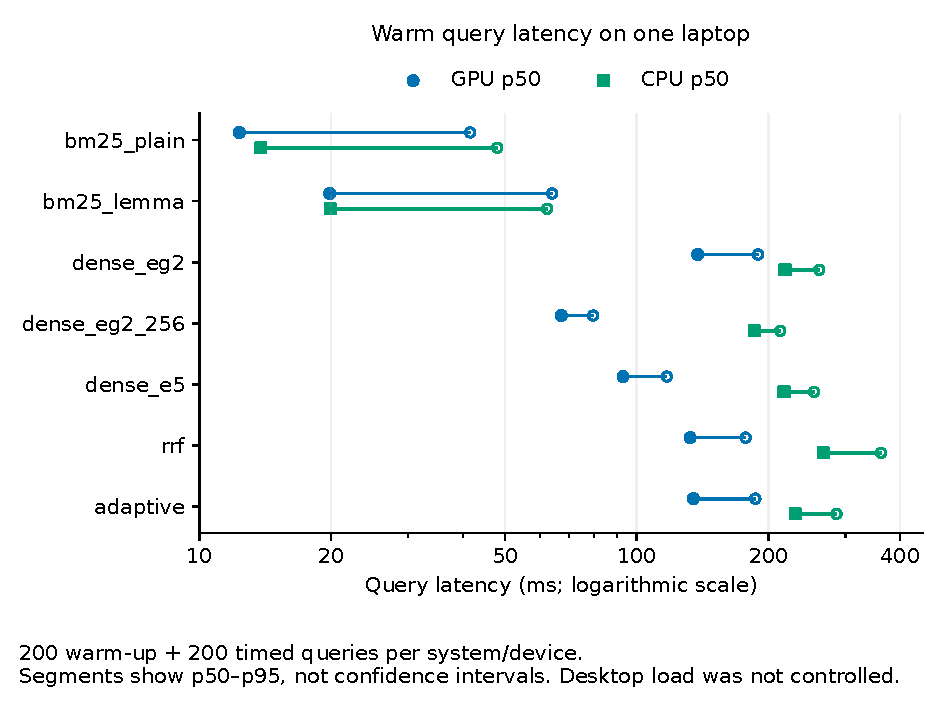
\includegraphics[width=\linewidth]{query_latency.pdf}
\caption{Query latency after a full warm-up. Markers show p50 and open endpoints p95, not confidence limits; the horizontal axis is logarithmic. Both passes include all 200 queries.}
\label{fig:query-latency}
\end{figure}

\begin{figure}[p]
\centering
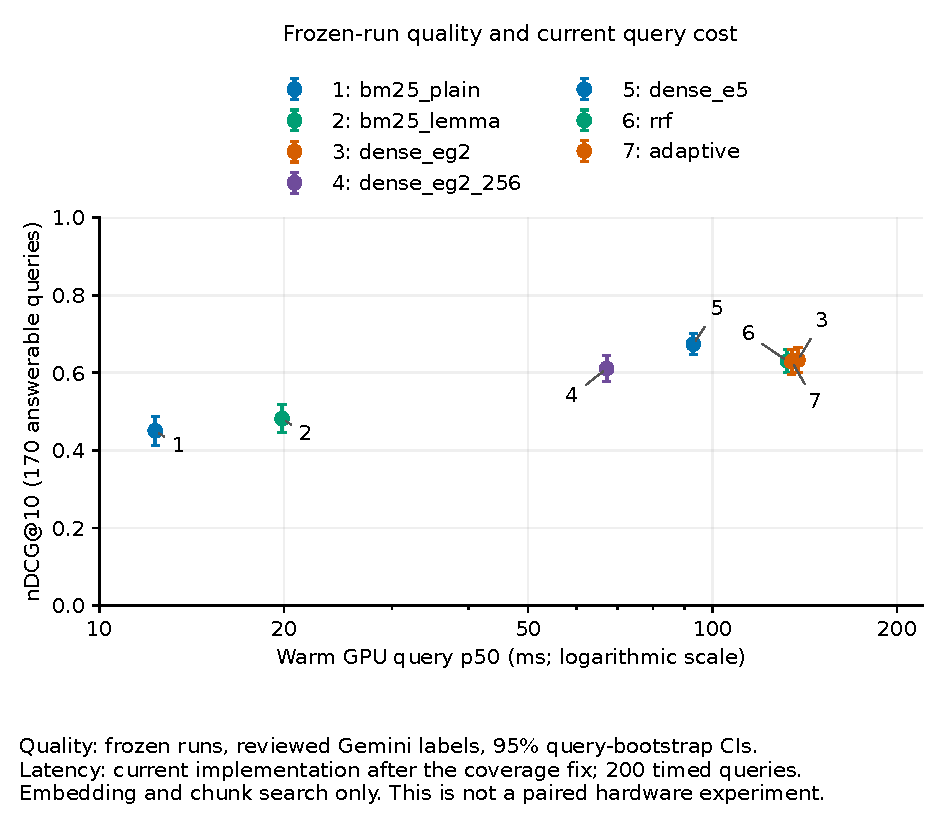
\includegraphics[width=\linewidth]{latency_quality.pdf}
\caption{Frozen original-run quality against current warm GPU query cost. Quality intervals use 170 answerable queries and reviewed Gemini labels; latency uses all 200 queries after the whole-word coverage correction. The two axes describe different code revisions, as disclosed in the control analysis, and do not form a paired hardware experiment. Document collapse is excluded from the timer.}
\label{fig:latency-quality}
\end{figure}
\else
\pending{Complete CPU/GPU query latency}
\fi
\ifpaperindexing
Table~\ref{tab:indexing} reports the GPU sample of 475 files and CPU sample of 95 files. Their compositions differ; chunks per second are descriptive throughput figures, and the ratio of wall times is not a paired hardware speedup.
\begin{table}[p]
\centering
\caption{Indexing into an empty database on two differently sized fixed samples. Counts refer to the files selected and chunks produced; RSS is the child-process peak. Sample disk includes database sidecars; full-index sizes count the main database files.}
\label{tab:indexing}
% Generated from primary=gemini_reviewed; see ../manifest.json for source SHA-256.
% indexing a fixed sample of the corpus with the archive CLI; source efficiency.json
\begingroup\small\setlength{\tabcolsep}{4pt}\renewcommand{\arraystretch}{1.3}
\noindent\begin{tabularx}{\linewidth}{@{}l*{7}{>{\centering\arraybackslash}X}@{}}
\toprule
Device & Files & Chunks & Seconds & Chunks/s & DB MiB & RSS MiB & VRAM +MiB \\
\midrule
GPU & 475 & 5\,155 & 106.1 & 48.58 & 59.9 & 2591 & 6816 \\
CPU & 95 & 1\,187 & 1395.1 & 0.85 & 13.6 & 2979 & 0 \\
\bottomrule
\end{tabularx}\endgroup

\par\medskip
% main database files; sample disk above includes sidecars
\begingroup\small\setlength{\tabcolsep}{4pt}\renewcommand{\arraystretch}{1.3}
\noindent\begin{tabularx}{\linewidth}{@{}l*{1}{>{\centering\arraybackslash}X}@{}}
\toprule
Full index & Main database MiB \\
\midrule
e5.sqlite3 & 1096.4 \\
full.sqlite3 & 1120.7 \\
noshort.sqlite3 & 1208.5 \\
plain.sqlite3 & 1094.7 \\
\bottomrule
\end{tabularx}\endgroup

\end{table}
\else
\pending{Complete CPU/GPU indexing measurements}
\fi

\subsection{Quantized retrieval}
\ifpapergguf
\begin{table}[p]
\centering
\caption{GGUF EG2 builds on the same text candidates as the bfloat16 reference. Query latency follows a full 200-query warm-up. Differences use reviewed Gemini labels and exploratory unadjusted paired tests; unjudged results are counted as non-relevant. File sizes are MiB.}
\label{tab:gguf}
% Generated from primary=gemini_reviewed; see ../manifest.json for source SHA-256.
% dense EG2 on the 4137 text documents; labels gemini_reviewed; source efficiency.json quantization
\begingroup\small\setlength{\tabcolsep}{4pt}\renewcommand{\arraystretch}{1.3}
\noindent\begin{tabularx}{\linewidth}{@{}l*{3}{>{\centering\arraybackslash}X}@{}}
\toprule
Build & File MiB & Chunks/s & Query p50 \\
\midrule
bf16 (SentenceTransformers) & -- & -- & -- \\
f16 & 532 & 46 & 76.7 \\
Q8\_0 & 296 & 48 & 86.0 \\
Q4\_K\_M & 173 & 46 & 83.6 \\
\bottomrule
\end{tabularx}\endgroup

\par\medskip
% dense EG2 on the 4137 text documents; labels gemini_reviewed; source efficiency.json quantization
\begingroup\small\setlength{\tabcolsep}{4pt}\renewcommand{\arraystretch}{1.3}
\noindent\begin{tabularx}{\linewidth}{@{}l*{4}{>{\centering\arraybackslash}X}@{}}
\toprule
Build & nDCG@10 & $\Delta$ [95\% CI] & p & Unjudged@10 \\
\midrule
bf16 (SentenceTransformers) & 0.631 & -- & -- & 0.003 \\
f16 & 0.631 & \shortstack{-0.001 \\ {\footnotesize[-0.005, +0.003]}} & 0.734 & 0.016 \\
Q8\_0 & 0.630 & \shortstack{-0.002 \\ {\footnotesize[-0.006, +0.003]}} & 0.504 & 0.018 \\
Q4\_K\_M & 0.613 & \shortstack{-0.018 \\ {\footnotesize[-0.030, -0.006]}} & 0.002 & 0.099 \\
\bottomrule
\end{tabularx}\endgroup

\par\medskip
% dense EG2 on the 4137 text documents; labels gemini_reviewed; source efficiency.json quantization; unjudged documents removed before ranking evaluation
\begingroup\small\setlength{\tabcolsep}{4pt}\renewcommand{\arraystretch}{1.3}
\noindent\begin{tabularx}{\linewidth}{@{}l*{3}{>{\centering\arraybackslash}X}@{}}
\toprule
Build & Condensed nDCG@10 & $\Delta$ [95\% CI] & p \\
\midrule
bf16 (SentenceTransformers) & 0.632 & -- & -- \\
f16 & 0.634 & \shortstack{+0.002 \\ {\footnotesize[-0.002, +0.006]}} & 0.297 \\
Q8\_0 & 0.633 & \shortstack{+0.000 \\ {\footnotesize[-0.004, +0.005]}} & 0.869 \\
Q4\_K\_M & 0.636 & \shortstack{+0.004 \\ {\footnotesize[-0.007, +0.015]}} & 0.454 \\
\bottomrule
\end{tabularx}\endgroup

\end{table}
\begin{figure}[p]
\centering
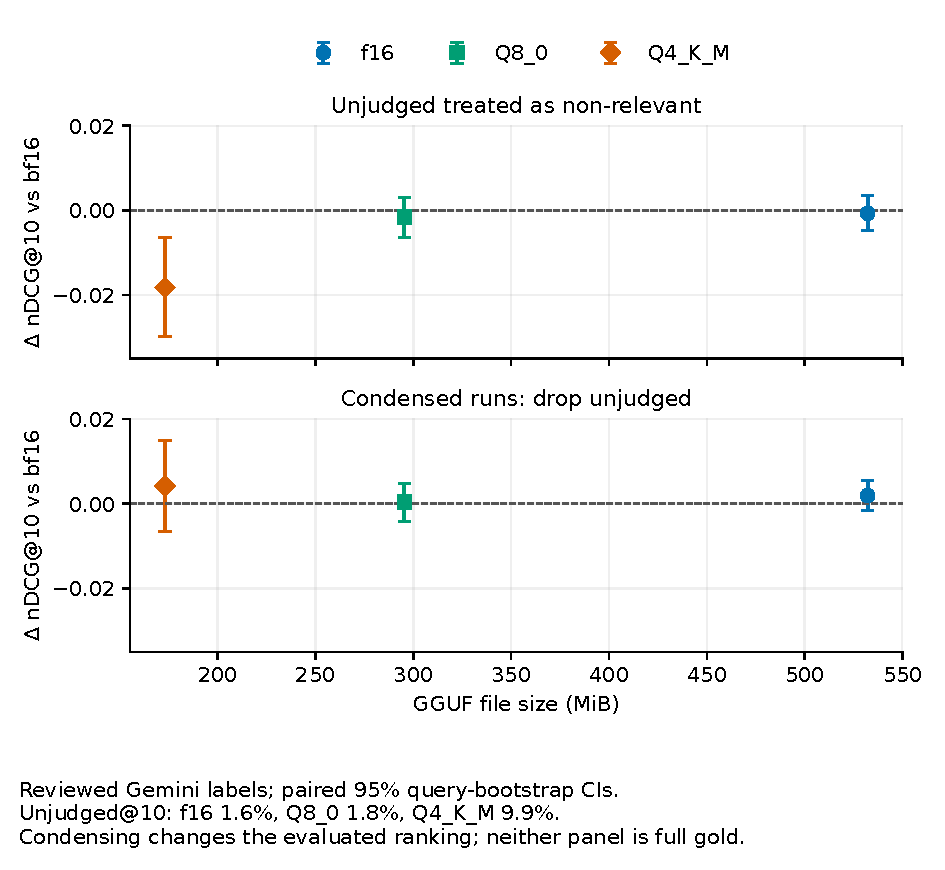
\includegraphics[width=\linewidth]{quantization_quality.pdf}
\caption{Paired nDCG@10 differences from bf16 EG2 versus GGUF file size on identical text candidates. The upper panel treats unjudged documents as non-relevant; the lower panel removes them. Error bars are 95\% query-bootstrap intervals. The dependence on judgement coverage prevents interpreting the upper Q4 difference as an isolated quantization effect.}
\label{fig:quantization-quality}
\end{figure}
Table~\ref{tab:gguf} reports retrieval quality, embedding throughput and local-server query latency. The separate cosine-reference experiment in the appendix does not substitute for these retrieval comparisons. The f16 and Q8 point differences from the bf16 reference are small, but intervals containing zero do not establish equivalence. For Q4, treating unjudged results as non-relevant gives a difference of $-0.018$ (95\% CI $[-0.030,-0.006]$); 9.9\% of its top-ten results are unjudged, compared with 0.3\% for the reference. On condensed runs the Q4 difference is $+0.004$ with an interval spanning zero. Removing unjudged results changes the evaluated ranking; it does not establish their relevance. Thus the frozen pool does not identify an intrinsic Q4 quality loss. These comparisons also change backend and numerical precision, not only quantization.
\else
\pending{GGUF retrieval-quality experiment incomplete; reference cosine measurements are in the appendix}
\fi

\subsection{Synthetic scaling}
\ifpaperann
\begin{table}[p]
\centering
\caption{Exact and approximate search on synthetic collections derived from the real vectors. Latencies are p50 milliseconds for a single query. HNSW cells show latency / recall@10 against exact search; construction time is seconds. This experiment measures chunk-vector search only.}
\label{tab:ann}
% Generated from primary=gemini_reviewed; see ../manifest.json for source SHA-256.
% p50 ms per single query; HNSW cells: p50 ms / strict-ID recall@10 against exact; source ann_scaling.json
\begingroup\small\setlength{\tabcolsep}{4pt}\renewcommand{\arraystretch}{1.3}
\noindent\begin{tabularx}{\linewidth}{@{}l*{5}{>{\centering\arraybackslash}X}@{}}
\toprule
Vectors & NumPy top-k & Faiss flat & HNSW build s & HNSW ef64 & HNSW ef256 \\
\midrule
100\,000 & 6.16 & 10.65 & 9 & 0.19 / 0.914 & 0.57 / 0.984 \\
300\,000 & 17.85 & 26.52 & 33 & 0.27 / 0.940 & 0.69 / 0.990 \\
1\,000\,000 & 51.78 & 75.83 & 187 & 0.29 / 0.904 & 0.97 / 0.991 \\
2\,000\,000 & 106.63 & 139.95 & 676 & 0.39 / 0.893 & 1.28 / 0.983 \\
\bottomrule
\end{tabularx}\endgroup

\par\medskip
% Actual semantic_scored path with candidate gather, full sort, pool400; no database polling; flat exact agreement / fraction at reference kth score within1e-6; source ann_reference_audit.json
\begingroup\small\setlength{\tabcolsep}{4pt}\renewcommand{\arraystretch}{1.3}
\noindent\begin{tabularx}{\linewidth}{@{}l*{3}{>{\centering\arraybackslash}X}@{}}
\toprule
Vectors & Archive path p50 ms & Flat ID agreement & Flat score threshold \\
\midrule
100\,000 & 60.84 & 1.000 & 1.000 \\
300\,000 & 166.80 & 1.000 & 1.000 \\
1\,000\,000 & 497.64 & 1.000 & 1.000 \\
2\,000\,000 & 2441.83 & 1.000 & 1.000 \\
\bottomrule
\end{tabularx}\endgroup

\par\smallskip
At 2\,000\,000 vectors, observed p50 is 106.6 ms for optimized NumPy top-k and 2441.8 ms for the archive vector path. HNSW ef256 is 1.28 ms at strict-ID recall@10 0.9825. These are sequential desktop-session measurements of different algorithms and output pools (10 versus 400), not paired hardware speedups or end-to-end interface latency.

\end{table}
\begin{figure}[p]
\centering
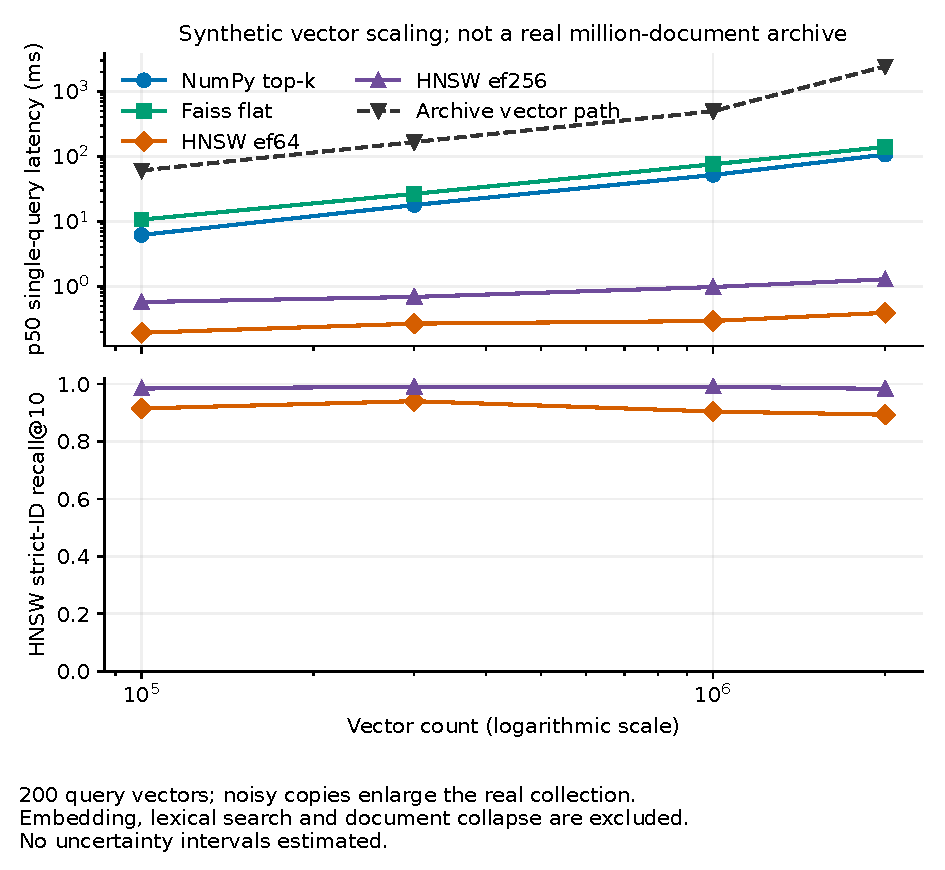
\includegraphics[width=\linewidth]{ann_scaling.pdf}
\caption{Vector-search latency and HNSW recall on synthetic enlarged collections. The latency axis is logarithmic, and no uncertainty intervals are estimated.}
\label{fig:ann-scaling}
\end{figure}
Table~\ref{tab:ann} separates exact vector-search cost from HNSW approximation. It excludes query embedding, lexical search and document collapse, and does not measure retrieval relevance on a real million-document archive.
\else
\pending{Complete exact/Faiss/HNSW scaling experiment}
\fi

\subsection{Additional target types}\label{sec:results-extension}
\ifpaperextension
The separate extension uses 50 Qwen-written queries targeting 20 documents, 15 tables and 15 repository files, evaluated with the corrected coverage rule. Initial Gemini labels and initial Gemma~4 12B labels are reported separately in Table~\ref{tab:extension}. The 50 records contain 49 distinct query wordings; one wording targets two files. They are not mixed into the original 200 or its primary relevance labels. GPT is comparison-only. Differences between the two query populations cannot identify self-preference because authorship, target type and difficulty also differ.
\begin{table}[p]
\centering
\caption{nDCG@10 and 95\% query-bootstrap intervals on the separate 50-query extension. Both label variants are initial assessments; neither is the original benchmark's reviewed primary variant.}
\label{tab:extension}
% Generated from primary=gemini_reviewed; see ../manifest.json for source SHA-256.
% nDCG@10, 95% query-bootstrap CI; separate 50-query extension; source extension.json
\begingroup\small\setlength{\tabcolsep}{4pt}\renewcommand{\arraystretch}{1.3}
\noindent\begin{tabularx}{\linewidth}{@{}l*{2}{>{\centering\arraybackslash}X}@{}}
\toprule
System & Gemini initial & Gemma 12B initial \\
\midrule
bm25\_plain & \shortstack{0.496 \\ {\footnotesize[0.404, 0.590]}} & \shortstack{0.507 \\ {\footnotesize[0.409, 0.604]}} \\
bm25\_lemma & \shortstack{0.523 \\ {\footnotesize[0.431, 0.617]}} & \shortstack{0.540 \\ {\footnotesize[0.443, 0.639]}} \\
dense\_eg2 & \shortstack{0.759 \\ {\footnotesize[0.697, 0.817]}} & \shortstack{0.769 \\ {\footnotesize[0.701, 0.832]}} \\
dense\_e5 & \shortstack{0.721 \\ {\footnotesize[0.654, 0.785]}} & \shortstack{0.730 \\ {\footnotesize[0.666, 0.790]}} \\
rrf & \shortstack{0.684 \\ {\footnotesize[0.619, 0.749]}} & \shortstack{0.696 \\ {\footnotesize[0.623, 0.766]}} \\
adaptive & \shortstack{0.756 \\ {\footnotesize[0.694, 0.814]}} & \shortstack{0.765 \\ {\footnotesize[0.697, 0.827]}} \\
adaptive-phrase & \shortstack{0.756 \\ {\footnotesize[0.694, 0.814]}} & \shortstack{0.765 \\ {\footnotesize[0.697, 0.827]}} \\
adaptive-ident & \shortstack{0.756 \\ {\footnotesize[0.694, 0.814]}} & \shortstack{0.765 \\ {\footnotesize[0.697, 0.827]}} \\
adaptive-short & \shortstack{0.756 \\ {\footnotesize[0.694, 0.814]}} & \shortstack{0.765 \\ {\footnotesize[0.697, 0.827]}} \\
dense\_eg2\_256 & \shortstack{0.713 \\ {\footnotesize[0.639, 0.782]}} & \shortstack{0.732 \\ {\footnotesize[0.662, 0.797]}} \\
\bottomrule
\end{tabularx}\endgroup

\end{table}

With initial Gemini labels, EG2 scores 0.759, adaptive fusion 0.756 and E5 0.721, compared with 0.523 for lemmatized BM25. With initial Gemma~4 12B labels the corresponding scores are 0.769, 0.765, 0.730 and 0.540. Adaptive exceeds both lexical baselines after Holm correction in both label variants; neither EG2 nor E5 is separated from adaptive by those tests. The changed point order of the dense encoders is cohort-specific evidence, not a comparison of overall difficulty with the original benchmark. GPT remains the most lenient judge on Qwen-written queries as well (mean grade 0.550 versus 0.379 for Gemini and 0.437 for Gemma), reinforcing that the initial GPT pattern does not identify query-author self-preference.

\ifpaperextensionunique
Keeping the lowest query ID per normalized wording removes q249, without selecting by retrieval score. Table~\ref{tab:extension-unique} reports this exploratory sensitivity. The 50-record intervals treat records as resampling units despite their shared wording; the separate sensitivity avoids that duplicate but does not make the sample representative.
\begin{table}[p]
\centering
\caption{Five principal systems on the unique-wording subset of the extension. Initial labels and query-bootstrap intervals; remaining systems and paired statistics are preserved in the result JSON.}
\label{tab:extension-unique}
% Generated from primary=gemini_reviewed; see ../manifest.json for source SHA-256.
Unique-wording sensitivity: 49 queries.
\par\smallskip
% keep lowest qid per normalized wording; source extension.json
\begingroup\small\setlength{\tabcolsep}{4pt}\renewcommand{\arraystretch}{1.3}
\noindent\begin{tabularx}{\linewidth}{@{}l*{2}{>{\centering\arraybackslash}X}@{}}
\toprule
System & Gemini initial & Gemma 12B initial \\
\midrule
bm25\_plain & \shortstack{0.503 \\ {\footnotesize[0.407, 0.597]}} & \shortstack{0.513 \\ {\footnotesize[0.414, 0.611]}} \\
bm25\_lemma & \shortstack{0.530 \\ {\footnotesize[0.439, 0.624]}} & \shortstack{0.546 \\ {\footnotesize[0.448, 0.646]}} \\
dense\_e5 & \shortstack{0.717 \\ {\footnotesize[0.649, 0.782]}} & \shortstack{0.724 \\ {\footnotesize[0.659, 0.786]}} \\
dense\_eg2 & \shortstack{0.757 \\ {\footnotesize[0.695, 0.813]}} & \shortstack{0.765 \\ {\footnotesize[0.698, 0.826]}} \\
adaptive & \shortstack{0.754 \\ {\footnotesize[0.692, 0.810]}} & \shortstack{0.760 \\ {\footnotesize[0.694, 0.821]}} \\
\bottomrule
\end{tabularx}\endgroup

\end{table}
\fi

\else
\pending{Separate 50-query document/table/code extension and its relevance assessments}
\fi

% Keep public-result floats ahead of the separate private-archive study.
\clearpage
% Private study: aggregate-only operational checks.
\section{Field study on the author's archive}\label{sec:field}

The private study runs the implemented adaptive search on the author's existing archive with three query sets written during system development. Their names (main, holdout7 and holdout11) are development labels, not evidence of an independently sampled or prospectively held-out user study. The sets contain 80, 86 and 214 queries respectively. No documents, query texts, paths, snippets or per-query outcomes are exported.

There are three operational checks. For an exact-item query, success means a returned chunk contains the expected phrase after whitespace and case normalization; ranks and reciprocal ranks are chunk-level. For a described-item query, success means the top five chunks include the expected project. For an absent-item query, success means lexical mode returns no result; this does not test abstention of dense search. The checks are weaker than independent document-relevance judgements. Each set and kind is summarized separately with query-bootstrap 95\% intervals; the sets are not pooled into a general performance estimate.

\ifpaperfield
\begin{table}[!htbp]
\centering
\caption{Operational checks on the private archive: counts, means and 95\% query-bootstrap intervals. Exact-item metrics use chunk ranks; described-item success checks the project; absent-item success checks lexical abstention. Only aggregates are exported.}
\label{tab:field}
% Generated from primary=gemini_reviewed; see ../manifest.json for source SHA-256.
Archive: 11\,394 documents, 902\,739 chunks.
\par\smallskip
% private archive aggregates only; exact ranks are chunk ranks; source field_aggregate.json
\begingroup\small\setlength{\tabcolsep}{4pt}\renewcommand{\arraystretch}{1.3}
\noindent\begin{tabularx}{\linewidth}{@{}l*{4}{>{\centering\arraybackslash}X}@{}}
\toprule
Set & Kind & Queries & Metric & Mean [95\% CI] \\
\midrule
holdout11 & exact & 192 & hit@1 & 0.672 [0.604, 0.740] \\
holdout11 & exact & 192 & hit@5 & 0.708 [0.641, 0.771] \\
holdout11 & exact & 192 & mrr@10 & 0.691 [0.627, 0.754] \\
holdout11 & absent & 10 & pass & 1.000 [1.000, 1.000] \\
holdout11 & described & 12 & hit@5 & 1.000 [1.000, 1.000] \\
holdout7 & exact & 64 & hit@1 & 0.641 [0.516, 0.750] \\
holdout7 & exact & 64 & hit@5 & 0.703 [0.594, 0.812] \\
holdout7 & exact & 64 & mrr@10 & 0.668 [0.557, 0.777] \\
holdout7 & absent & 10 & pass & 1.000 [1.000, 1.000] \\
holdout7 & described & 12 & hit@5 & 1.000 [1.000, 1.000] \\
main & exact & 66 & hit@1 & 0.697 [0.576, 0.803] \\
main & exact & 66 & hit@5 & 0.727 [0.621, 0.833] \\
main & exact & 66 & mrr@10 & 0.709 [0.598, 0.813] \\
main & absent & 8 & pass & 1.000 [1.000, 1.000] \\
main & described & 6 & hit@5 & 1.000 [1.000, 1.000] \\
\bottomrule
\end{tabularx}\endgroup

\end{table}
Table~\ref{tab:field} describes this deployment and these development queries. All-success samples produce degenerate percentile-bootstrap intervals of [1,1]; these are not population guarantees. Its intervals describe resampling within a set; they do not account for tuning on the archive, query selection or variation between people.
\else
\pending{Private field study aggregates not yet available}
\fi

% Flush result floats before interpretation and references.
\clearpage
% Interpretation of completed results; no new measurements or labels.
\section{Discussion}\label{sec:discussion}

\paragraph{Morphology (RQ1).}
Corrected lemma expansion increases BM25 nDCG@10 by 0.031 under the primary labels, with a paired 95\% interval from 0.013 to 0.051. This supports a gain for this query set under these assessments. The weaker evidence under Gemma~4 12B limits a judge-independent conclusion. The earlier decrease before the analyzer fix also illustrates an implementation dependency: expansion with an incorrectly guessed lemma can change retrieval in the opposite direction. The result concerns the tested analyzer rule and corpus, rather than morphology as a universally beneficial operation.

\paragraph{Fusion and technical queries (RQ2--RQ3).}
Adaptive fusion exceeds BM25 on the primary endpoint but has no detected advantage over EG2 or RRF. E5 has the highest mean nDCG@10, including in the control with the same text candidates. The absence of a Holm-significant E5--adaptive contrast does not establish equal effectiveness. The phrase-reranking ablation is numerically identical to the full system on the frozen runs; the identifier and short-fragment ablations likewise provide no evidence of an improvement on this sample. A rule can address a plausible failure case without that case occurring often enough here to improve the aggregate metric. A general recommendation about the fusion rule would therefore require independently written queries and broader target coverage.

\paragraph{Changing target coverage.}
The separate extension produces a different ordering: EG2 and adaptive fusion have higher point estimates than E5 under its initial Gemini labels. Query authorship, target formats and the assessment variant also change between cohorts. The extension therefore cannot identify which factor produces that difference, and its means should not be treated as a before/after improvement over the original benchmark. Retaining the 50-record analysis beside the deterministic 49-wording sensitivity preserves the original data while making the duplicated wording visible.

\paragraph{Multimodal matching (RQ4).}
Caption--image and transcript--recording tasks test cross-modal matching in two languages using source-dataset pairings. Image recall at one is 0.857 for Ukrainian captions and 0.889 for Russian captions among 1\,000 images. These outcomes are distinct from the model-judged text-retrieval results. For speech, using the same transcript as query and indexed text is a ceiling condition; even cross-lingual transcripts are parallel source sentences. Neither task establishes effectiveness for a person's paraphrase, a long recording or arbitrary photographs. The tasks support the implemented modality connection within their stated matching conditions.

\paragraph{Quantization and judgement coverage (RQ5).}
The ordinary Q4 comparison has a negative point difference, while its condensed-list comparison does not show the same loss; 9.9\% of Q4 top-10 results are unjudged. The frozen pool therefore cannot identify an intrinsic Q4 relevance loss from the ordinary score. Conversely, the small f16/Q8 differences and intervals spanning zero do not establish equivalence. Backend and precision change together, and the 21 PDF-page rows also change input modality. Quality, file size and encoding cost should be read jointly with these coverage and implementation conditions, rather than as an isolated causal effect of quantization.

\paragraph{The cost of the implemented search path.}
At two million synthetic vectors, the actual archive-ranking path has median time about 2\,442~ms, while the optimized NumPy top-10 reference takes about 107~ms. The paths perform different work: the archive method gathers candidates, fully sorts scores and constructs 400 tuples. This gap identifies implementation work that a matrix-product-only description would miss. HNSW with search depth 256 takes about 1.28~ms and has strict-ID recall@10 of 0.9825 on this synthetic collection. These sequential desktop measurements are not an end-to-end or paired speedup estimate, and the recall need not transfer to a real archive of that size. They motivate approximate indexing and candidate-selection work as future engineering directions.

\paragraph{Assessment and practical interpretation.}
Judge agreement, target checks and deliberate no-answer queries diagnose assessment behaviour without establishing human relevance validity. The Gemini review retains dependence on the original assessors and visible grades, so label sensitivity accompanies the point estimates. An independent human study and queries written by people seeking their own documents remain future validation; they are not reported as completed here. The private-archive checks show that the system can satisfy the author's operational expectations in that deployment, while their development reuse prevents a user-effectiveness claim. Taken together, the evidence supports an inspectable account of quality and cost in one constructed benchmark and one deployment, with the strongest comparisons conditional on their labels, populations and measurement boundaries.

% Limitations and threats to validity.
\section{Limitations and threats to validity}\label{sec:limitations}

\subsection{Corpus and queries}
\uapar{} imitates a personal archive with public material: Wikipedia articles stand in for notes and rendered articles for office documents, so the text is more uniform and better edited than real notes, and nothing in it is truly personal. The 200 queries were written by one model under written rules, not by people looking for their own documents, and every answerable target is a note. The separate 50-query extension targets documents, tables and repository files (Section~\ref{sec:results-extension}), but is again model-written. It contains 49 distinct wordings, so the 50 records are not fully independent; a deterministic unique-wording sensitivity is reported separately. The no-answer queries have no lexical match by construction, which decides the lexical systems' result on them in advance. Topics follow the author's interests; a different archive could favour different systems.

\subsection{Model-generated relevance labels}
Text relevance labels are generated by language models rather than an independent human panel. Agreement, target-document checks and deliberately unanswerable queries provide diagnostic evidence but are not a complete gold standard. Gemini and Gemma may share errors because they share a provider. Reviewing disagreements with Gemini cannot remove this dependence; it also exposes the reviewer to the initial grades. We therefore preserve the original labels and report the sensitivity of retrieval metrics and system ordering to the judge and to the review. The primary judge was selected after examining judge diagnostics, a post hoc methodological choice. This edition deliberately includes no human relevance audit. Its text-retrieval conclusions therefore remain conditional on the model judgements; independent human validation is future work.

\subsection{Query and candidate coverage}
Although the corpus is heterogeneous, all authored answerable targets in the original 200-query set are notes. The separate extension adds a small sample of documents, tables and repository files. Neither set establishes general quality for arbitrary target formats, images or recordings. The E5 baseline searches a smaller text-only document universe, whereas the EG2 indexes include media. The control on identical candidates (Table~\ref{tab:encoder-control}) changes EG2's nDCG@10 by $-0.0015$, a small point effect in this control. This does not remove all candidate-coverage uncertainty: the control runs were not pooled, and 0.29\% of their top-10 documents are unjudged.

Only the union of system top-10 results is fully judged. Relevant documents outside that pool may exist. Recall at 100 is therefore relative to the known relevant pool; treating unjudged documents as nonrelevant can favour pooled systems and does not estimate exhaustive corpus recall. A failure to reject a performance difference does not establish equivalence.

\subsection{Single-author field study}
The field study (Section~\ref{sec:field}) uses one person's archive and query sets that the author wrote during development of the system, partly to test it; they are not a random sample of real information needs, and the system was tuned on the same archive. Its numbers show behaviour in deployment, not generalizable effectiveness.

\subsection{Measurements}
All costs come from one laptop in an ordinary desktop session, with other programs running; the load before each step is logged but not controlled. The query timer includes embedding and chunk search but excludes document collapse, path resolution and interface rendering. Process-level resource counters span the whole measured pass, including collapse, so their scope differs from the per-query timer. CPU indexing was measured on a fifth of the GPU sample. The scaling experiment uses synthetic vectors derived from the real ones, and HNSW recall on them need not equal recall on a real collection of that size.

\subsection{Construct validity}
Judges see the title and the first 1\,200 characters of a document, not the whole document, so a document relevant only further down can be graded too low; the same snippet is shown for every system, so the bias does not favour one system directly but favours documents whose relevance shows early. Grades 0/1/2 compress a judgement that people make differently: a model's ``partly relevant'' is not a person's. The primary metric, nDCG@10 over pooled labels, rewards systems for ranking judged-relevant documents high; it does not measure whether a person finds what they remember faster, which is what an archive search is for.

\subsection{Source-pair matching tasks}
Image and speech tasks identify the paired source item or sentence. Those pairings do not exhaustively judge every semantically related candidate. Captions and parallel transcripts also differ from independently paraphrased archive queries. The reported point estimates have no computed confidence intervals.

% Release identifiers remain pending author decisions; example DOIs are not reused.
\section{Data and code availability}\label{sec:availability}

\paragraph{Research artifacts.}
The public author-review release provides executable source, saved result JSON, manuscript sources, generated tables and figures, and both PDFs at \url{https://github.com/cyberdid/archive-index-public}, tag \code{paper-author-review-2026-10-23}. No software/data or preprint DOI has been assigned. The generated-table manifest binds numerical artifacts to their source hashes. The public package supports rebuilding tables and PDFs from saved results. The full frozen corpus, query/run/assessment inputs and their 14-stage replay are retained in a separate research archive; they are not redistributed in this release while third-party attribution and scope review remain pending. Exact end-to-end statistical replay therefore requires those separately held inputs. The corpus-construction and evaluation scripts are public.

\paragraph{Reproduction.}
The isolated \path{paper/run_all.sh} runner distinguishes a saved-result rendering pass from a full frozen-input statistical replay. The completed full replay has 14 stages and reproduces ten reports, canonical qrels and recorded ANN input hashes. Physical cost, multimodal, ANN and private-field measurements are imported artifacts in this replay, not newly repeated experiments. The recorded 315 implementation tests, including a locally cached real-model integration check, address implementation behaviour separately. Observed environment specifications and hash-locked requirements accompany the code; a fresh full CUDA installation is not claimed. Rebuilding tables or PDFs does not by itself repeat model grading or physical measurements.

\paragraph{Source policy and attribution.}
The corpus manifest records source URL, collected licence label and SHA-256 for every file. Notes and rendered documents derive from Ukrainian and Russian Wikipedia (CC~BY-SA~4.0); the 150 selected data.gov.ua tables carry CC~BY labels. Crossmodal-3600 images retain per-image CC~BY~2.0 attribution, with CC~BY~4.0 captions; FLEURS recordings and transcripts carry CC~BY~4.0. Repository selection accepted MIT or Apache-2.0 API labels; the collected code repositories are labelled MIT in the manifest. That repository-level label is not a per-asset licence determination. Embedded third-party notices remain applicable: the attribution inventory records, among other cases, the Rubik font's SIL~OFL notice, a pinned missing-license supplement, and an application-terms scope question. Original notices, attribution files and the audit in \path{paper/corpus/LICENSES.md} are preserved. The final redistribution review of third-party material remains pending.

\paragraph{Licensing.}
The original executable source is licensed under Apache License~2.0. Article text, original figures and experimental records are licensed under Creative Commons Attribution~4.0 International (\url{https://creativecommons.org/licenses/by/4.0/}), to the extent the author holds the relevant rights. The licensing guide distinguishes these materials from third-party corpus assets and dependencies, which retain their own terms.

\paragraph{Private data and release inspection.}
Only aggregate operational checks are exported from the author's archive; its documents, query texts, paths, snippets and index are excluded. The release guard checks filenames, known marker bytes, decoded JSON, extracted PDF text/metadata and supported compressed content. Four investigated public word/name collisions require explicit source evidence and exact file hashes; full private-query and home-path markers have no exception. These checks do not constitute a universal privacy guarantee or OCR inspection of images. The existing private Git history is not an appropriate public release; publication requires a separately reviewed export.

\paragraph{Models and software.}
The experiment records identify EmbeddingGemma~2 (\code{google/embeddinggemma-2}, revision \code{914f7f8}), multilingual-E5-large (\code{intfloat/multilingual-e5-large}), the llama.cpp/GGUF builds and every judging model. Package, model and command fingerprints remain tied to their recorded runs. Model weights are not included in the research export.

\paragraph{AI-assisted work.}
Model-written queries and model relevance assessments are described in Section~\ref{sec:uapar} and the separate extension analysis; GPT grades remain comparison-only. Claude and Codex assisted implementation and manuscript preparation, and the Scientific Agent Skills workflow~\citep{kassis2026skills} informed source and claim checks. The author is responsible for the study design, interpretations, references and final declarations. No AI system is an author. This edition includes no human text-relevance audit; source-dataset multimodal pairings and implementation checks do not replace one.

% Conclusions are conditional on the observed archive, labels and measurement scope.
\section{Conclusion}\label{sec:conclusion}

This study makes the retrieval choices in archive-index inspectable through a constructed multilingual collection, frozen queries and runs, preserved model assessments and generated reports. Under the primary reviewed Gemini labels on 170 answerable queries, mean nDCG@10 is 0.674 for E5, 0.633 for EG2, 0.629 for adaptive fusion, 0.482 for lemmatized BM25 and 0.450 for plain BM25. Adaptive fusion exceeds BM25 after correction, while these data do not establish an advantage over EG2 or RRF. Evidence for the morphology gain depends on the assessor, and the separate extension shows that the point ordering of encoders can change with the cohort.

The broader result is a measured account of implementation and evaluation trade-offs. Quantized retrieval depends on judgement coverage and input/backend differences; synthetic scaling distinguishes optimized vector selection from the actual archive-ranking path; multimodal tasks and private-archive checks answer narrower questions than human text-retrieval effectiveness. The findings concern a constructed benchmark evaluated with model-generated relevance labels. Independent human assessments, independently written information needs and evaluation across archives remain future validation before general claims about personal-archive search.


\bibliographystyle{plainnat}
\bibliography{../refs}

\appendix
\clearpage
\section{Detailed measured results}
The following fragments are generated from the same result files as the main tables. Their source hashes and current primary relevance variant are recorded in \path{generated/manifest.json}.
\subsection{Assessment status and scope}
% Generated from primary=gemini_reviewed; see ../manifest.json for source SHA-256.
\begingroup\raggedright
Judging: Gemini within-model reviewed. Metrics: 170 answerable queries; no-answer queries: 30.
\par
R@100 is pool-relative; judgments are incomplete, not full gold. Gemini and Gemma12 share a provider family. Gemini review is within-model. GPT is excluded from principal tables and figures.
\par
gemini: 5572 graded pairs.
\par
gemma4-12b: 5572 graded pairs.
\par
Initial disagreements: 1091/5572; linear-weighted Cohen kappa: 0.652.
\par
Targets: total=170, in pool=134, outside pool=36. Target-grade denominator=134.
\par
The manifest describes collected files, not all of them are indexable by archive-index.
\par
The E5 baseline uses text-only input; its document universe differs from the multimodal EG2 indexes.
\par
All 170 authored answerable query targets are notes; findings do not establish retrieval quality for targets in every archive format.
\par
Raw chunks include lexical-only rows. Text-collection vector counts restrict collections to wiki, docs, tables and code; they include image-rendered PDF pages. Text-vector counts exclude image/audio input hashes.
\par\endgroup

\subsection{Collected and indexed populations}
% Generated from primary=gemini_reviewed; see ../manifest.json for source SHA-256.
% Collected files and indexed documents are different populations; E5 text-only and full indexes do not share the same document universe.
\begingroup\small\setlength{\tabcolsep}{4pt}\renewcommand{\arraystretch}{1.3}
\noindent\begin{tabularx}{\linewidth}{@{}l*{1}{>{\centering\arraybackslash}X}@{}}
\toprule
Population & Count \\
\midrule
Manifest files & 7070 \\
Queries (all) & 200 \\
e5 index documents & 4137 \\
full index documents & 6054 \\
noshort index documents & 6054 \\
plain index documents & 6054 \\
e5: raw chunks & 94970 \\
e5: vectors & 84767 \\
e5: text-collection vectors & 84767 \\
full: raw chunks & 96908 \\
full: vectors & 86726 \\
full: text-collection vectors & 84788 \\
noshort: raw chunks & 97652 \\
noshort: vectors & 87441 \\
noshort: text-collection vectors & 85503 \\
plain: raw chunks & 96908 \\
plain: vectors & 86726 \\
plain: text-collection vectors & 84788 \\
\bottomrule
\end{tabularx}\endgroup

\clearpage
\subsection{Ablations}
% Generated from primary=gemini_reviewed; see ../manifest.json for source SHA-256.
% Means with 95% bootstrap CI; n=170. R@100 is pool-relative under incomplete judgments. Significance: paired comparison against adaptive only, \(p_{\mathrm{Holm}}<0.05\).
\begingroup\small\setlength{\tabcolsep}{4pt}\renewcommand{\arraystretch}{1.3}
\noindent\begin{tabularx}{\linewidth}{@{}l*{3}{>{\centering\arraybackslash}X}@{}}
\toprule
System & nDCG@10 & R@100\textsuperscript{pool} & RR@10 \\
\midrule
adaptive & \shortstack{0.629 \\ {\footnotesize[0.596, 0.660]}} & \shortstack{0.908 \\ {\footnotesize[0.887, 0.928]}} & \shortstack{0.866 \\ {\footnotesize[0.826, 0.905]}} \\
adaptive-phrase & \shortstack{0.629 \\ {\footnotesize[0.596, 0.660]}} & \shortstack{0.908 \\ {\footnotesize[0.887, 0.928]}} & \shortstack{0.866 \\ {\footnotesize[0.826, 0.905]}} \\
adaptive-ident & \shortstack{0.629 \\ {\footnotesize[0.597, 0.661]}} & \shortstack{0.912 \\ {\footnotesize[0.892, 0.931]}} & \shortstack{0.866 \\ {\footnotesize[0.826, 0.905]}} \\
adaptive-short & \shortstack{0.629 \\ {\footnotesize[0.597, 0.660]}} & \shortstack{0.908 \\ {\footnotesize[0.887, 0.928]}} & \shortstack{0.866 \\ {\footnotesize[0.826, 0.905]}} \\
dense\_eg2\_256 & \shortstack{0.611 \\ {\footnotesize[0.577, 0.643]}} & \shortstack{0.888\textsuperscript{\textdagger} \\ {\footnotesize[0.863, 0.911]}} & \shortstack{0.873 \\ {\footnotesize[0.830, 0.913]}} \\
\bottomrule
\end{tabularx}\endgroup

\par\medskip
% Means with 95% bootstrap CI; n=170. R@100 is pool-relative under incomplete judgments. Significance: paired comparison against adaptive only, \(p_{\mathrm{Holm}}<0.05\).
\begingroup\small\setlength{\tabcolsep}{4pt}\renewcommand{\arraystretch}{1.3}
\noindent\begin{tabularx}{\linewidth}{@{}l*{2}{>{\centering\arraybackslash}X}@{}}
\toprule
System & Success@1 & Success@5 \\
\midrule
adaptive & \shortstack{0.782 \\ {\footnotesize[0.718, 0.841]}} & \shortstack{0.971 \\ {\footnotesize[0.941, 0.994]}} \\
adaptive-phrase & \shortstack{0.782 \\ {\footnotesize[0.718, 0.841]}} & \shortstack{0.971 \\ {\footnotesize[0.941, 0.994]}} \\
adaptive-ident & \shortstack{0.782 \\ {\footnotesize[0.718, 0.841]}} & \shortstack{0.971 \\ {\footnotesize[0.941, 0.994]}} \\
adaptive-short & \shortstack{0.782 \\ {\footnotesize[0.718, 0.841]}} & \shortstack{0.971 \\ {\footnotesize[0.941, 0.994]}} \\
dense\_eg2\_256 & \shortstack{0.818 \\ {\footnotesize[0.759, 0.871]}} & \shortstack{0.953 \\ {\footnotesize[0.918, 0.982]}} \\
\bottomrule
\end{tabularx}\endgroup

\par\smallskip
{\footnotesize \textdagger: p\textsubscript{Holm}<0.05, adaptive; R@100: pool-relative.}

\clearpage
\subsection{Query categories}
% Generated from primary=gemini_reviewed; see ../manifest.json for source SHA-256.
% nDCG@10; source subgroup 95% bootstrap CIs; primary=gemini_reviewed.
\begingroup\small\setlength{\tabcolsep}{4pt}\renewcommand{\arraystretch}{1.3}
\noindent\begin{tabularx}{\linewidth}{@{}l*{2}{>{\centering\arraybackslash}X}@{}}
\toprule
System & Known item & Topical \\
\midrule
bm25\_plain & \shortstack{0.475 \\ {\footnotesize[0.397, 0.552]}} & \shortstack{0.351 \\ {\footnotesize[0.296, 0.407]}} \\
bm25\_lemma & \shortstack{0.524 \\ {\footnotesize[0.451, 0.594]}} & \shortstack{0.388 \\ {\footnotesize[0.338, 0.438]}} \\
dense\_eg2 & \shortstack{0.617 \\ {\footnotesize[0.549, 0.683]}} & \shortstack{0.568 \\ {\footnotesize[0.513, 0.619]}} \\
dense\_e5 & \shortstack{0.729 \\ {\footnotesize[0.682, 0.773]}} & \shortstack{0.662 \\ {\footnotesize[0.617, 0.706]}} \\
rrf & \shortstack{0.639 \\ {\footnotesize[0.584, 0.690]}} & \shortstack{0.564 \\ {\footnotesize[0.517, 0.609]}} \\
adaptive & \shortstack{0.612 \\ {\footnotesize[0.542, 0.680]}} & \shortstack{0.568 \\ {\footnotesize[0.513, 0.619]}} \\
adaptive-phrase & \shortstack{0.612 \\ {\footnotesize[0.542, 0.680]}} & \shortstack{0.568 \\ {\footnotesize[0.513, 0.619]}} \\
adaptive-ident & \shortstack{0.612 \\ {\footnotesize[0.542, 0.680]}} & \shortstack{0.568 \\ {\footnotesize[0.513, 0.619]}} \\
adaptive-short & \shortstack{0.612 \\ {\footnotesize[0.543, 0.681]}} & \shortstack{0.569 \\ {\footnotesize[0.514, 0.620]}} \\
dense\_eg2\_256 & \shortstack{0.596 \\ {\footnotesize[0.527, 0.664]}} & \shortstack{0.539 \\ {\footnotesize[0.479, 0.598]}} \\
\bottomrule
\end{tabularx}\endgroup

\par\medskip
% nDCG@10; source subgroup 95% bootstrap CIs; primary=gemini_reviewed.
\begingroup\small\setlength{\tabcolsep}{4pt}\renewcommand{\arraystretch}{1.3}
\noindent\begin{tabularx}{\linewidth}{@{}l*{2}{>{\centering\arraybackslash}X}@{}}
\toprule
System & Technical & Cross-lingual \\
\midrule
bm25\_plain & \shortstack{0.649 \\ {\footnotesize[0.597, 0.702]}} & \shortstack{0.351 \\ {\footnotesize[0.273, 0.427]}} \\
bm25\_lemma & \shortstack{0.651 \\ {\footnotesize[0.595, 0.706]}} & \shortstack{0.388 \\ {\footnotesize[0.302, 0.472]}} \\
dense\_eg2 & \shortstack{0.785 \\ {\footnotesize[0.746, 0.823]}} & \shortstack{0.582 \\ {\footnotesize[0.512, 0.650]}} \\
dense\_e5 & \shortstack{0.663 \\ {\footnotesize[0.606, 0.716]}} & \shortstack{0.639 \\ {\footnotesize[0.563, 0.709]}} \\
rrf & \shortstack{0.779 \\ {\footnotesize[0.734, 0.824]}} & \shortstack{0.554 \\ {\footnotesize[0.486, 0.619]}} \\
adaptive & \shortstack{0.772 \\ {\footnotesize[0.732, 0.810]}} & \shortstack{0.582 \\ {\footnotesize[0.512, 0.650]}} \\
adaptive-phrase & \shortstack{0.772 \\ {\footnotesize[0.732, 0.810]}} & \shortstack{0.582 \\ {\footnotesize[0.512, 0.650]}} \\
adaptive-ident & \shortstack{0.775 \\ {\footnotesize[0.736, 0.813]}} & \shortstack{0.582 \\ {\footnotesize[0.512, 0.650]}} \\
adaptive-short & \shortstack{0.772 \\ {\footnotesize[0.732, 0.810]}} & \shortstack{0.580 \\ {\footnotesize[0.510, 0.648]}} \\
dense\_eg2\_256 & \shortstack{0.757 \\ {\footnotesize[0.716, 0.796]}} & \shortstack{0.579 \\ {\footnotesize[0.508, 0.648]}} \\
\bottomrule
\end{tabularx}\endgroup

\clearpage
\subsection{Query languages}
% Generated from primary=gemini_reviewed; see ../manifest.json for source SHA-256.
% nDCG@10; source subgroup 95% bootstrap CIs; primary=gemini_reviewed.
\begingroup\small\setlength{\tabcolsep}{4pt}\renewcommand{\arraystretch}{1.3}
\noindent\begin{tabularx}{\linewidth}{@{}l*{2}{>{\centering\arraybackslash}X}@{}}
\toprule
System & Russian & Ukrainian \\
\midrule
bm25\_plain & \shortstack{0.421 \\ {\footnotesize[0.368, 0.474]}} & \shortstack{0.466 \\ {\footnotesize[0.417, 0.515]}} \\
bm25\_lemma & \shortstack{0.480 \\ {\footnotesize[0.428, 0.531]}} & \shortstack{0.483 \\ {\footnotesize[0.436, 0.530]}} \\
dense\_eg2 & \shortstack{0.633 \\ {\footnotesize[0.582, 0.683]}} & \shortstack{0.633 \\ {\footnotesize[0.592, 0.672]}} \\
dense\_e5 & \shortstack{0.664 \\ {\footnotesize[0.612, 0.712]}} & \shortstack{0.679 \\ {\footnotesize[0.647, 0.710]}} \\
rrf & \shortstack{0.624 \\ {\footnotesize[0.579, 0.668]}} & \shortstack{0.634 \\ {\footnotesize[0.596, 0.671]}} \\
adaptive & \shortstack{0.623 \\ {\footnotesize[0.572, 0.674]}} & \shortstack{0.631 \\ {\footnotesize[0.591, 0.670]}} \\
adaptive-phrase & \shortstack{0.623 \\ {\footnotesize[0.572, 0.674]}} & \shortstack{0.631 \\ {\footnotesize[0.591, 0.670]}} \\
adaptive-ident & \shortstack{0.625 \\ {\footnotesize[0.574, 0.676]}} & \shortstack{0.631 \\ {\footnotesize[0.591, 0.670]}} \\
adaptive-short & \shortstack{0.623 \\ {\footnotesize[0.572, 0.674]}} & \shortstack{0.632 \\ {\footnotesize[0.591, 0.670]}} \\
dense\_eg2\_256 & \shortstack{0.637 \\ {\footnotesize[0.584, 0.689]}} & \shortstack{0.597 \\ {\footnotesize[0.553, 0.640]}} \\
\bottomrule
\end{tabularx}\endgroup

\subsection{Quantization reference}
The reference measures cosine agreement of embeddings on 20 texts and CPU seconds per text. It does not measure retrieval-quality loss or establish production latency.
\par\medskip
% Generated from primary=gemini_reviewed; see ../manifest.json for source SHA-256.
% External quantization reference: embedding cosine agreement, not retrieval quality. Point estimates; no CI available. Prompt counts: f16=20, Q8_0=20, Q4_K_M=20
\begingroup\small\setlength{\tabcolsep}{4pt}\renewcommand{\arraystretch}{1.3}
\noindent\begin{tabularx}{\linewidth}{@{}l*{4}{>{\centering\arraybackslash}X}@{}}
\toprule
GGUF & Mean cosine & Worst cosine & MB & CPU s/text \\
\midrule
f16 & 0.99995 & 0.99994 & 532.1 & 0.061 \\
Q8\_0 & 0.99972 & 0.99892 & 295.5 & 0.069 \\
Q4\_K\_M & 0.99043 & 0.98503 & 173.3 & 0.053 \\
\bottomrule
\end{tabularx}\endgroup

\par

\clearpage
% Preserved provenance, moved from the introduction.
\section{Implementation corrections and protocol changes}\label{sec:intro-history}
Implementation corrections and assessment-protocol changes were identified during development. The record below distinguishes corrections applied before the frozen runs from the later coverage control.
\begin{enumerate}
\item \emph{Lemmas invented by the other language's analyzer.} Words without Ukrainian-only letters went through both analyzers, and the one that did not know the word invented a lemma (\emph{навчанню}$\to$\emph{навчаннить}). In the first target-document diagnostic, lemmatized BM25 found the target in the top 10 for 45.3\% of the answerable queries against 49.4\% without lemmas; after the fix it found 50.0\%. All reported runs use the fixed analyzer.
\item \emph{Rebuilt terms differed from indexed terms} for pictures and sound, so an ablation index made by rebuilding terms was not identical to one built from scratch. Fixed before the runs used here.
\item \emph{A relative corpus path} stored documents twice in an ablation index. Caught and fixed before any run was evaluated.
\item \emph{Heading-only judge snippets.} In the first judging sheet, 393 of 5\,572 pairs showed the judge under 200 characters, mostly a title and a source line. The snippet was changed to the beginning of the document before any judging was used.
\item \emph{Query authorship.} The first query file named Claude as the author of queries that GPT-6-Luna wrote; it was corrected before judging, and GPT grades were then kept out of the labels.
\item \emph{Substring coverage in the adaptive rule.} The test for an exact phrase counted substrings (\code{36} inside \code{1366}). It was found after the runs were frozen; the frozen runs are reported and the corrected rule is reported beside them (it changes the top~10 for one query of 200).
\item \emph{Change of relevance protocol.} The plan named Claude as the primary judge. After the judge diagnostics and before the reported aggregate retrieval comparison was computed, the author chose Gemini as the primary judge. A later partial Claude pass is deferred at the author's request and is excluded from all reported analyses. This is a post hoc decision and is reported as one.
\end{enumerate}

\end{document}
